\chapter{Vectors, Matrices and Linear Systems}\label{ch:linear-algebra}

\begin{chapterintro}
In first-year physics a vector is an arrow: a displacement, a velocity, a force, with two or three components. This chapter keeps everything you know about arrows (adding, scaling, the dot product, length, perpendicularity) and drops one restriction, the number of components. A list of 400 numbers turns out to obey the same rules as a list of three, and once you accept that, a great deal of computation becomes geometry. "How far is my prediction from the truth?" becomes the length of a difference vector. "Is my prediction shaped like the truth?" becomes the angle between two vectors. "Can I find coefficients that reproduce these data exactly?" becomes the question of whether a system of linear equations has a solution, and how many.

We also introduce matrices. A matrix is a rectangular table of numbers, but its real meaning is a rule that turns one vector into another in a straight-line (linear) way. We learn to multiply matrices, to undo them (the inverse), to solve the equations they define by elimination, to measure how many independent pieces of information they carry (the rank), and to compute the determinant. We end by treating functions themselves as vectors with very many components, which is exactly what a computer does when it stores a wavefunction on a grid.

Where this shows up in the paper \cite{soniR1}: the fitted correction $\delta V(x)=\sum_k c_k\cos(k\pi x/L)$ of Sec.~II~C is a basis expansion with a coefficient vector $c$; the residuals $r_n=\tilde t_n-E_n$ form a residual vector; the sensitivity $A_{nk}=\int|\psi_n|^2\cos(k\pi x/L)\,\dd x$ is a matrix with one row per level and one column per basis function; every rms in every table is the length of a vector divided by the square root of its number of components; and statements such as ``at 900 coefficients on 400 zeros the least-squares problem is underdetermined'' (Sec.~IV) are statements about linear systems with more unknowns than equations.
\end{chapterintro}

\begin{prerequisites}
\item Chapter~\ref{ch:complex}: complex numbers $z=a+ib$, the complex conjugate $z^*=a-ib$, the modulus $\abs{z}$ with $\abs{z}^2=z^*z$, Euler's formula $e^{i\theta}=\cos\theta+i\sin\theta$.
\item First-year physics: vectors in two and three dimensions, components, the dot product $\bm a\cdot\bm b=a_xb_x+a_yb_y+a_zb_z$, the magnitude $\abs{\bm a}=\sqrt{\bm a\cdot\bm a}$, the relation $\bm a\cdot\bm b=\abs{\bm a}\abs{\bm b}\cos\theta$, and the cross product.
\item Calculus: the integral as a limit of Riemann sums, integration by parts, the identities $\cos^2\theta+\sin^2\theta=1$, $\sin^2\theta=\tfrac12(1-\cos2\theta)$ and $\cos A\cos B=\tfrac12[\cos(A-B)+\cos(A+B)]$.
\item Appendix A (Python) for the code listings: arrays, \texttt{@} for matrix products, \texttt{numpy.linalg}.
\end{prerequisites}

%======================================================================
\section{From arrows to lists of numbers}\label{sec:linear-algebra-lists}

A displacement in the laboratory is written $\bm r=(x,y,z)$: three numbers, in a fixed order. Nothing in the rules for adding displacements or stretching them depends on there being exactly three. Add two displacements and you add their components one by one; double a displacement and you double each component. So we make the following definition.

\paragraph{Definition.} A \emph{real vector with $n$ components} is an ordered list of $n$ real numbers,
\begin{equation}
\bm v=(v_1,v_2,\dots,v_n).
\label{eq:linear-algebra-vector}
\end{equation}
The number $v_j$ is the $j$-th \emph{component}. The set of all such lists is called $\mathbb R^n$ (read ``R-n''). When we want to stress the arrangement we write the list as a column,
\[
\bm v=\begin{pmatrix}v_1\\ v_2\\ \vdots\\ v_n\end{pmatrix}.
\]
In this chapter vectors are printed in bold. The paper prints them in plain type: its coefficient vector is simply $c$.

Two examples from the running examples of this book:
\begin{itemize}
\item The heights of the first ten zeta zeros (running example RE1),
\[
\bm t=(14.134725,\ 21.022040,\ 25.010858,\ 30.424876,\ 32.935062,\ 37.586178,\ 40.918719,\ 43.327073,\ 48.005151,\ 49.773832),
\]
form a vector in $\mathbb R^{10}$. You do not need to know yet where these numbers come from (Chapter~\ref{ch:zeta} explains); here they are just ten ordered numbers.
\item In the paper's fits, the correction to the potential is described by $M$ numbers $c_0,c_1,\dots,c_{M-1}$, so the coefficient vector $\bm c$ lies in $\mathbb R^{M}$; for $M=400$ it has 400 components. (The paper starts this index at $0$, not $1$; we return to this in a pitfall below.)
\end{itemize}

\paragraph{Addition and scaling.} For $\bm u,\bm v\in\mathbb R^n$ and a real number $\alpha$ (a \emph{scalar}) we define
\begin{align}
\bm u+\bm v &= (u_1+v_1,\ u_2+v_2,\ \dots,\ u_n+v_n), \label{eq:linear-algebra-add}\\
\alpha\bm v &= (\alpha v_1,\ \alpha v_2,\ \dots,\ \alpha v_n). \label{eq:linear-algebra-scale}
\end{align}
The \emph{zero vector} $\bm 0=(0,\dots,0)$ satisfies $\bm v+\bm 0=\bm v$, and $-\bm v=(-1)\bm v$ satisfies $\bm v+(-\bm v)=\bm 0$. Because each component is an ordinary real number, the familiar rules carry over component by component. For example, the distributive rule $\alpha(\bm u+\bm v)=\alpha\bm u+\alpha\bm v$ holds because its $j$-th component reads $\alpha(u_j+v_j)=\alpha u_j+\alpha v_j$, which is the distributive law for real numbers. In the same way $\bm u+\bm v=\bm v+\bm u$ and $(\bm u+\bm v)+\bm w=\bm u+(\bm v+\bm w)$.

\paragraph{Linear combinations.} An expression
\begin{equation}
\alpha_1\bm v_1+\alpha_2\bm v_2+\dots+\alpha_k\bm v_k
\label{eq:linear-algebra-lincomb}
\end{equation}
with scalars $\alpha_i$ and vectors $\bm v_i$ is called a \emph{linear combination} of the $\bm v_i$. Almost everything in this chapter is about linear combinations: which vectors can be built from which, and with what coefficients.

\Cref{fig:linear-algebra-vectors} (left) shows addition in $\mathbb R^2$, where you can still draw arrows: $\bm u+\bm v$ is the diagonal of the parallelogram with sides $\bm u$ and $\bm v$. In $\mathbb R^{400}$ you cannot draw the picture, but every algebraic statement we prove holds there just as well, and the two-dimensional picture remains an honest guide to intuition.

\begin{figure}[htbp]\centering
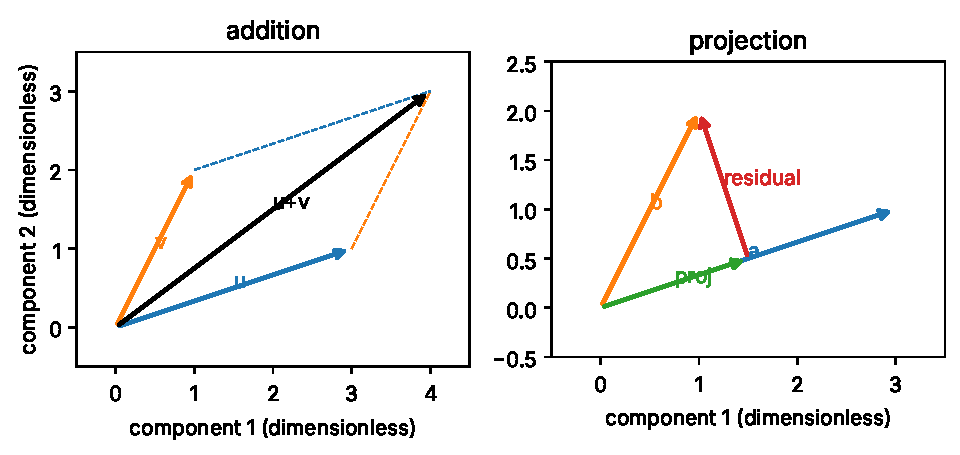
\includegraphics[width=0.85\linewidth]{figs/linear-algebra_vectors.pdf}
\caption{Left: addition of $\bm u=(3,1)$ and $\bm v=(1,2)$ gives the diagonal $\bm u+\bm v=(4,3)$ of the parallelogram they span. Right: the projection of $\bm b=(1,2)$ onto the direction of $\bm a=(3,1)$ is $(1.5,0.5)$; the residual $\bm b-(1.5,0.5)=(-0.5,1.5)$ is perpendicular to $\bm a$. Components are dimensionless.}
\label{fig:linear-algebra-vectors}
\end{figure}

\begin{checkpoint}
A model predicts the vector $\bm p=(1.0,\,2.0,\,3.0)$ and the truth is $\bm d=(1.5,\,1.5,\,3.5)$. What is the error vector $\bm p-\bm d$?
\end{checkpoint}
\checkanswer{$\bm p-\bm d=(1.0-1.5,\ 2.0-1.5,\ 3.0-3.5)=(-0.5,\ 0.5,\ -0.5)$, computed component by component from \cref{eq:linear-algebra-add,eq:linear-algebra-scale} with $\bm p-\bm d=\bm p+(-1)\bm d$.}

\begin{keyideas}
\item A vector in $\mathbb R^n$ is an ordered list of $n$ real numbers; addition and scaling act component by component.
\item All the algebraic rules of 3D vectors hold in $\mathbb R^n$ because they hold for each component.
\item A linear combination $\sum_i\alpha_i\bm v_i$ is the basic object of linear algebra.
\end{keyideas}

%======================================================================
\section{Length, angle and the inner product}\label{sec:linear-algebra-inner}

\subsection{The inner product and the norm}

In three dimensions $\bm a\cdot\bm b=a_xb_x+a_yb_y+a_zb_z$. The obvious generalization is the following.

\paragraph{Definition.} The \emph{inner product} (or dot product) of $\bm u,\bm v\in\mathbb R^n$ is
\begin{equation}
\bm u\cdot\bm v=\sum_{j=1}^{n}u_jv_j=u_1v_1+u_2v_2+\dots+u_nv_n .
\label{eq:linear-algebra-dot}
\end{equation}
The \emph{norm} (length) of $\bm v$ is
\begin{equation}
\norm{\bm v}=\sqrt{\bm v\cdot\bm v}=\sqrt{v_1^2+v_2^2+\dots+v_n^2},
\label{eq:linear-algebra-norm}
\end{equation}
and the \emph{distance} between $\bm u$ and $\bm v$ is $\norm{\bm u-\bm v}$.

Three properties follow directly from \cref{eq:linear-algebra-dot}:
\begin{enumerate}
\item Symmetry: $\bm u\cdot\bm v=\bm v\cdot\bm u$, because $u_jv_j=v_ju_j$ for each $j$.
\item Linearity: $\bm u\cdot(\alpha\bm v+\beta\bm w)=\sum_ju_j(\alpha v_j+\beta w_j)=\alpha\sum_ju_jv_j+\beta\sum_ju_jw_j=\alpha\,\bm u\cdot\bm v+\beta\,\bm u\cdot\bm w$.
\item Positivity: $\bm v\cdot\bm v=\sum_jv_j^2\ge0$, and it equals zero only if every $v_j=0$, because a sum of squares of real numbers vanishes only when each square does.
\end{enumerate}
A vector with $\norm{\bm v}=1$ is a \emph{unit vector}. Any nonzero vector can be \emph{normalized}: $\hat{\bm v}=\bm v/\norm{\bm v}$ has norm $\norm{\bm v}/\norm{\bm v}=1$, using $\norm{\alpha\bm v}=\sqrt{\sum_j\alpha^2v_j^2}=\abs{\alpha}\norm{\bm v}$.

\subsection{The rms is a norm in disguise}

The paper scores every prediction by an ``rms'', a root mean square error. If a model makes errors $e_1,\dots,e_n$ (in the paper, each error is measured in units of the local mean spacing between zeros, Chapter~\ref{ch:counting-zeros}), then
\begin{equation}
\rms(\bm e)=\sqrt{\frac1n\sum_{j=1}^ne_j^2}=\frac{\norm{\bm e}}{\sqrt n}.
\label{eq:linear-algebra-rms}
\end{equation}
The second equality is \cref{eq:linear-algebra-norm} with the factor $1/n$ moved outside the square root as $1/\sqrt n$. So the rms is the length of the error vector, rescaled so that it does not grow merely because you have more components. This is why rms values for 100 held-out zeros and for 500 held-out zeros can be compared.

\begin{sample}{Norm and rms of a residual vector}
A fit leaves residuals $\bm r=(0.3,\,-0.1,\,0.2,\,-0.4)$ (in mean spacings) on four levels. Find $\norm{\bm r}$ and $\rms(\bm r)$.

\textbf{Step 1:} Square and add the components: $\bm r\cdot\bm r=0.09+0.01+0.04+0.16=0.30$.

\textbf{Step 2:} The norm is $\norm{\bm r}=\sqrt{0.30}=0.5477$.

\textbf{Step 3:} By \cref{eq:linear-algebra-rms}, $\rms(\bm r)=\norm{\bm r}/\sqrt4=\sqrt{0.30/4}=\sqrt{0.075}$.

\[
\boxed{\norm{\bm r}=0.5477,\qquad \rms(\bm r)=0.2739.}
\]
\end{sample}

\subsection{The Cauchy--Schwarz inequality and angles}

In three dimensions $\bm a\cdot\bm b=\abs{\bm a}\abs{\bm b}\cos\theta$, so $\abs{\bm a\cdot\bm b}\le\abs{\bm a}\abs{\bm b}$. We want to define an angle in $\mathbb R^n$, and for that we first need the same inequality there, proved without pictures.

\paragraph{Theorem (Cauchy--Schwarz).} For all $\bm u,\bm v\in\mathbb R^n$,
\begin{equation}
\abs{\bm u\cdot\bm v}\le\norm{\bm u}\,\norm{\bm v}.
\label{eq:linear-algebra-cs}
\end{equation}

\emph{Proof.} If $\bm v=\bm 0$ both sides are zero. Otherwise, for every real number $\lambda$ the vector $\bm u-\lambda\bm v$ has a non-negative squared norm. Expanding with the linearity and symmetry properties,
\begin{align*}
0\le\norm{\bm u-\lambda\bm v}^2 &=(\bm u-\lambda\bm v)\cdot(\bm u-\lambda\bm v)\\
&=\bm u\cdot\bm u-\lambda\,\bm u\cdot\bm v-\lambda\,\bm v\cdot\bm u+\lambda^2\,\bm v\cdot\bm v\\
&=\norm{\bm u}^2-2\lambda\,\bm u\cdot\bm v+\lambda^2\norm{\bm v}^2 .
\end{align*}
This holds for every $\lambda$; choose $\lambda=(\bm u\cdot\bm v)/\norm{\bm v}^2$. Then
\begin{align*}
0&\le\norm{\bm u}^2-2\frac{(\bm u\cdot\bm v)^2}{\norm{\bm v}^2}+\frac{(\bm u\cdot\bm v)^2}{\norm{\bm v}^4}\norm{\bm v}^2\\
&=\norm{\bm u}^2-\frac{(\bm u\cdot\bm v)^2}{\norm{\bm v}^2}.
\end{align*}
Multiplying by $\norm{\bm v}^2>0$ gives $(\bm u\cdot\bm v)^2\le\norm{\bm u}^2\norm{\bm v}^2$, and taking the non-negative square root gives \cref{eq:linear-algebra-cs}. $\square$

Because of \cref{eq:linear-algebra-cs}, for nonzero vectors the ratio $\bm u\cdot\bm v/(\norm{\bm u}\norm{\bm v})$ lies between $-1$ and $+1$. We may therefore \emph{define} the angle $\theta$ between them by
\begin{equation}
\cos\theta=\frac{\bm u\cdot\bm v}{\norm{\bm u}\,\norm{\bm v}},\qquad 0\le\theta\le\pi .
\label{eq:linear-algebra-angle}
\end{equation}
In $\mathbb R^3$ this is the ordinary angle; in $\mathbb R^n$ it is the definition. Two vectors are \emph{orthogonal} if $\bm u\cdot\bm v=0$ (angle $\pi/2$).

\paragraph{Triangle inequality.} $\norm{\bm u+\bm v}\le\norm{\bm u}+\norm{\bm v}$. Proof: $\norm{\bm u+\bm v}^2=\norm{\bm u}^2+2\,\bm u\cdot\bm v+\norm{\bm v}^2\le\norm{\bm u}^2+2\norm{\bm u}\norm{\bm v}+\norm{\bm v}^2=(\norm{\bm u}+\norm{\bm v})^2$, where the inequality is \cref{eq:linear-algebra-cs}. Take square roots of both (non-negative) sides.

\begin{checkpoint}
Are $(1,2,3)$ and $(3,0,-1)$ orthogonal? Is $(1,1,1,1)$ orthogonal to $(1,-1,1,-1)$?
\end{checkpoint}
\checkanswer{Yes to both: $1\cdot3+2\cdot0+3\cdot(-1)=0$, and $1-1+1-1=0$.}

\subsection{Prediction, truth and the angle between them}

The paper reports, for each prediction, both an rms and a correlation. Linear algebra shows that these measure different things and how they are related.

Let $\bm d$ be the vector of true values (say, true fluctuations of the zeros) and $\bm p$ the vector of predicted values. The \emph{null} prediction is $\bm p=\bm 0$ (``no fluctuation''); its error vector is $-\bm d$ and its error norm is $\norm{\bm d}$. For any prediction, expanding as in the Cauchy--Schwarz proof,
\begin{align}
\norm{\bm p-\bm d}^2&=\norm{\bm p}^2-2\,\bm p\cdot\bm d+\norm{\bm d}^2 \label{eq:linear-algebra-errid}\\
&=\norm{\bm p}^2-2\norm{\bm p}\norm{\bm d}\cos\theta+\norm{\bm d}^2,\qquad\text{(by \cref{eq:linear-algebra-angle})}\nonumber
\end{align}
with $\theta$ the angle between $\bm p$ and $\bm d$. The prediction beats the null exactly when $\norm{\bm p-\bm d}^2<\norm{\bm d}^2$, that is, when $\norm{\bm p}^2<2\norm{\bm p}\norm{\bm d}\cos\theta$. For $\bm p\neq\bm 0$ divide by $\norm{\bm p}$:
\begin{equation}
\norm{\bm p-\bm d}<\norm{\bm d}\quad\Longleftrightarrow\quad\norm{\bm p}<2\norm{\bm d}\cos\theta .
\label{eq:linear-algebra-beatnull}
\end{equation}
Two consequences follow at once.
\begin{itemize}
\item If $\cos\theta\le0$, the right side of \cref{eq:linear-algebra-beatnull} is $\le0$, which no positive $\norm{\bm p}$ can be below. So \emph{every nonzero prediction that is orthogonal or anti-aligned to the truth is worse than predicting nothing.}
\item If we keep the direction $\hat{\bm p}$ fixed and choose the length $\alpha$ of $\bm p=\alpha\hat{\bm p}$ to minimize the error, \cref{eq:linear-algebra-errid} reads $\alpha^2-2\alpha\norm{\bm d}\cos\theta+\norm{\bm d}^2$, a parabola in $\alpha$ with minimum at $\alpha=\norm{\bm d}\cos\theta$ (set the derivative $2\alpha-2\norm{\bm d}\cos\theta$ to zero). The minimum value is $\norm{\bm d}^2-\norm{\bm d}^2\cos^2\theta=\norm{\bm d}^2\sin^2\theta$, so the best achievable error in that direction is
\begin{equation}
\min_\alpha\norm{\alpha\hat{\bm p}-\bm d}=\norm{\bm d}\sin\theta .
\label{eq:linear-algebra-sintheta}
\end{equation}
\end{itemize}

The Pearson correlation of statistics (Chapter~\ref{ch:probability}) is $\cos\theta$ computed after subtracting from each vector the mean of its components. If $\bar p=\frac1n\sum_jp_j$ and $\bm 1=(1,\dots,1)$, then
\begin{equation}
\corr(\bm p,\bm d)=\frac{(\bm p-\bar p\bm 1)\cdot(\bm d-\bar d\bm 1)}{\norm{\bm p-\bar p\bm 1}\,\norm{\bm d-\bar d\bm 1}} .
\label{eq:linear-algebra-corr}
\end{equation}
By \cref{eq:linear-algebra-cs} applied to the centered vectors, $-1\le\corr\le1$. When both vectors already have mean close to zero, as fluctuations do, the correlation and the $\cos\theta$ of \cref{eq:linear-algebra-angle} are close, and the geometry above applies approximately to rms and corr.

\begin{sample}{Right shape, wrong size; right size, wrong shape}
The truth is $\bm d=(1,-1,2,-2)$. Compare the null, the prediction $\bm p=(0.5,-0.5,1,-1)$, and the prediction $\bm q=(2,-2,-1,1)$, by rms error and correlation.

\textbf{Step 1 (null):} error vector $-\bm d$, $\norm{\bm d}^2=1+1+4+4=10$, so $\rms=\sqrt{10/4}=1.5811$.

\textbf{Step 2 ($\bm p$):} $\bm p=\tfrac12\bm d$, so $\bm p\cdot\bm d=\tfrac12\cdot10=5$, $\norm{\bm p}=\tfrac12\sqrt{10}$, and $\cos\theta=5/(\tfrac12\sqrt{10}\cdot\sqrt{10})=1$. Both vectors have mean zero, so $\corr=1$. The error is $\bm p-\bm d=(-0.5,0.5,-1,1)$ with squared norm $2.5$, so $\rms=\sqrt{2.5/4}=0.7906$.

\textbf{Step 3 ($\bm q$):} $\bm q\cdot\bm d=2+2-2-2=0$, mean of $\bm q$ is zero, so $\corr=0$; $\norm{\bm q}^2=4+4+1+1=10=\norm{\bm d}^2$. By \cref{eq:linear-algebra-errid}, $\norm{\bm q-\bm d}^2=10-0+10=20$, so $\rms=\sqrt{20/4}=2.2361$, which is $\sqrt2$ times the null.

\[
\boxed{\text{null } 1.5811;\quad \bm p:\ \rms=0.7906,\ \corr=1;\quad \bm q:\ \rms=2.2361,\ \corr=0.}
\]
The perfectly shaped prediction has a large error because its amplitude is wrong; the uncorrelated prediction of the right amplitude is worse than saying nothing.
\end{sample}

\begin{keyideas}
\item $\bm u\cdot\bm v=\sum_ju_jv_j$, $\norm{\bm v}=\sqrt{\bm v\cdot\bm v}$; rms $=\norm{\bm e}/\sqrt n$ (\cref{eq:linear-algebra-rms}).
\item Cauchy--Schwarz (\cref{eq:linear-algebra-cs}) lets us define angles in $\mathbb R^n$ (\cref{eq:linear-algebra-angle}).
\item Correlation is the cosine of the angle between centered vectors; a prediction with $\cos\theta\le0$ cannot beat the null (\cref{eq:linear-algebra-beatnull}), and the best rescaled prediction has error $\norm{\bm d}\sin\theta$ (\cref{eq:linear-algebra-sintheta}).
\end{keyideas}

%======================================================================
\section{Complex vectors}\label{sec:linear-algebra-complex}

Quantum wavefunctions (Chapter~\ref{ch:schrodinger}) are complex, and in the paper's Sec.~II~E the eigenvectors of a non-Hermitian matrix are complex. So we need vectors whose components are complex numbers. Addition and scaling (now by complex scalars) work exactly as before. The inner product needs one change.

\begin{checkpoint}
Using the real formula \cref{eq:linear-algebra-dot} without change, compute $\bm u\cdot\bm u$ for $\bm u=(1,i)$. Would this make a sensible ``length squared''?
\end{checkpoint}
\checkanswer{$1\cdot1+i\cdot i=1+i^2=0$. A nonzero vector would have length zero, which is useless as a length. The formula must be modified.}

Recall from Chapter~\ref{ch:complex} that for a complex number $z$, $z^*z=\abs{z}^2\ge0$, with equality only when $z=0$. So we put a conjugate on the first factor.

\paragraph{Definition.} For $\bm u,\bm v\in\mathbb C^n$ (lists of $n$ complex numbers) the inner product is
\begin{equation}
\langle\bm u,\bm v\rangle=\sum_{j=1}^nu_j^*v_j ,
\label{eq:linear-algebra-cinner}
\end{equation}
and the norm is $\norm{\bm v}=\sqrt{\langle\bm v,\bm v\rangle}=\sqrt{\sum_j\abs{v_j}^2}$.

This is the physicists' convention (conjugate on the first slot), the one used with the bra--ket notation $\braket{u}{v}$ of Chapter~\ref{ch:schrodinger}. Some mathematics books conjugate the second slot instead; the content is the same. For real vectors $u_j^*=u_j$ and \cref{eq:linear-algebra-cinner} reduces to \cref{eq:linear-algebra-dot}.

\paragraph{Properties.}
\begin{enumerate}
\item Conjugate symmetry: $\langle\bm u,\bm v\rangle^*=\sum_j(u_j^*v_j)^*=\sum_ju_jv_j^*=\langle\bm v,\bm u\rangle$, using $(ab)^*=a^*b^*$ and $(a^*)^*=a$.
\item Linearity in the second slot: $\langle\bm u,\alpha\bm v+\beta\bm w\rangle=\alpha\langle\bm u,\bm v\rangle+\beta\langle\bm u,\bm w\rangle$, exactly as in the real case.
\item Conjugate-linearity in the first slot: $\langle\alpha\bm u,\bm v\rangle=\sum_j(\alpha u_j)^*v_j=\alpha^*\langle\bm u,\bm v\rangle$.
\item Positivity: $\langle\bm v,\bm v\rangle=\sum_j\abs{v_j}^2\ge0$, zero only for $\bm v=\bm 0$.
\end{enumerate}
Property 1 implies that $\langle\bm v,\bm v\rangle$ equals its own conjugate, so it is real, as a squared length must be. The Cauchy--Schwarz inequality $\abs{\langle\bm u,\bm v\rangle}\le\norm{\bm u}\norm{\bm v}$ still holds (Problem~21 asks you to prove it). Two complex vectors are orthogonal if $\langle\bm u,\bm v\rangle=0$.

\begin{sample}{A complex inner product}
Let $\bm u=(1+i,\ 2)$ and $\bm v=(i,\ 1-i)$. Compute $\langle\bm u,\bm v\rangle$, $\langle\bm v,\bm u\rangle$, $\norm{\bm u}$, $\norm{\bm v}$, and check Cauchy--Schwarz.

\textbf{Step 1:} Conjugate the components of $\bm u$: $(1-i,\ 2)$.

\textbf{Step 2:} $\langle\bm u,\bm v\rangle=(1-i)\,i+2(1-i)=i-i^2+2-2i=i+1+2-2i=3-i$.

\textbf{Step 3:} By conjugate symmetry $\langle\bm v,\bm u\rangle=(3-i)^*=3+i$. (Directly: $(-i)(1+i)+(1+i)\cdot2=-i+1+2+2i=3+i$.)

\textbf{Step 4:} $\norm{\bm u}^2=\abs{1+i}^2+\abs{2}^2=2+4=6$; $\norm{\bm v}^2=\abs{i}^2+\abs{1-i}^2=1+2=3$.

\textbf{Step 5:} $\abs{3-i}^2=9+1=10\le6\cdot3=18$. The inequality holds.
\[
\boxed{\langle\bm u,\bm v\rangle=3-i,\quad \norm{\bm u}=\sqrt6,\quad\norm{\bm v}=\sqrt3.}
\]
\end{sample}

\begin{pitfall}
In \texttt{numpy}, \texttt{np.dot(u, v)} and \texttt{u @ v} do \emph{not} conjugate anything. For complex vectors the inner product \cref{eq:linear-algebra-cinner} is \texttt{np.vdot(u, v)}, which conjugates its first argument, or equivalently \texttt{u.conj() @ v}. Using \texttt{u @ u} for a complex norm gives nonsense such as the $0$ of the checkpoint above.
\end{pitfall}

\begin{pycode}
import numpy as np
u = np.array([1+1j, 2])
v = np.array([1j, 1-1j])
print(np.vdot(u, v))           # (3-1j): conjugates u
print(u @ v)                   # no conjugate: a different number
print(np.linalg.norm(u)**2)    # 6.0 (norm conjugates correctly)
r = np.array([0.3, -0.1, 0.2, -0.4])
print(np.linalg.norm(r), np.sqrt(np.mean(r**2)))   # 0.5477, 0.2739
\end{pycode}

\begin{keyideas}
\item For complex vectors, $\langle\bm u,\bm v\rangle=\sum_ju_j^*v_j$; the conjugate makes $\langle\bm v,\bm v\rangle=\sum_j\abs{v_j}^2$ real and non-negative.
\item $\langle\bm u,\bm v\rangle^*=\langle\bm v,\bm u\rangle$; linear in the second slot, conjugate-linear in the first.
\end{keyideas}

%======================================================================
\section{Bases, orthogonality and projection}\label{sec:linear-algebra-basis}

\subsection{Independence, span and basis}

\paragraph{Definitions.} Vectors $\bm v_1,\dots,\bm v_k$ are \emph{linearly independent} if the only solution of
\[
\alpha_1\bm v_1+\dots+\alpha_k\bm v_k=\bm 0
\]
is $\alpha_1=\dots=\alpha_k=0$. Otherwise they are \emph{dependent}: one of them (any one with a nonzero $\alpha_i$) can be written as a linear combination of the others. The \emph{span} of the $\bm v_i$ is the set of all their linear combinations. A \emph{basis} of $\mathbb R^n$ (or $\mathbb C^n$) is a set of independent vectors whose span is the whole space.

The \emph{standard basis} is $\bm e_1=(1,0,\dots,0)$, $\bm e_2=(0,1,0,\dots,0)$, \dots, $\bm e_n=(0,\dots,0,1)$. It spans everything because $\bm v=v_1\bm e_1+\dots+v_n\bm e_n$, and it is independent because $\sum\alpha_j\bm e_j=(\alpha_1,\dots,\alpha_n)$ is zero only if every $\alpha_j=0$.

\begin{beyond}
\textbf{Taken on trust: dimension.} Every basis of $\mathbb R^n$ or $\mathbb C^n$ contains exactly $n$ vectors, and any $n$ independent vectors form a basis. The number $n$ is the \emph{dimension}. The proof is not hard but needs a careful counting argument (the ``exchange lemma''); see Strang \cite{strang}, Ch.~3, or Riley, Hobson and Bence \cite{rhb}, Ch.~8. We use the consequence that more than $n$ vectors in $\mathbb R^n$ are always dependent.
\end{beyond}

\subsection{Orthogonal sets and components}

\paragraph{Theorem.} Nonzero, mutually orthogonal vectors are linearly independent.

\emph{Proof.} Suppose $\sum_j\alpha_j\bm v_j=\bm 0$ with $\langle\bm v_k,\bm v_j\rangle=0$ for $j\neq k$. Take the inner product of both sides with $\bm v_k$:
\[
0=\langle\bm v_k,\textstyle\sum_j\alpha_j\bm v_j\rangle=\sum_j\alpha_j\langle\bm v_k,\bm v_j\rangle=\alpha_k\norm{\bm v_k}^2 .
\]
Since $\bm v_k\ne\bm 0$, $\norm{\bm v_k}^2>0$, so $\alpha_k=0$. This holds for every $k$. $\square$

An \emph{orthonormal} basis is a basis $\bm e_1,\dots,\bm e_n$ with $\langle\bm e_j,\bm e_k\rangle=\delta_{jk}$, where the Kronecker delta $\delta_{jk}$ is $1$ if $j=k$ and $0$ otherwise. In an orthonormal basis, components are found by inner products. If $\bm v=\sum_ja_j\bm e_j$, then
\begin{equation}
\langle\bm e_k,\bm v\rangle=\sum_ja_j\langle\bm e_k,\bm e_j\rangle=\sum_ja_j\delta_{jk}=a_k .
\label{eq:linear-algebra-components}
\end{equation}
And the squared norm is the sum of squared components (a finite form of Parseval's theorem, which Chapter~\ref{ch:fourier-series} meets for functions):
\begin{equation}
\norm{\bm v}^2=\Big\langle\sum_ja_j\bm e_j,\sum_ka_k\bm e_k\Big\rangle=\sum_j\sum_ka_j^*a_k\delta_{jk}=\sum_k\abs{a_k}^2 .
\label{eq:linear-algebra-parseval}
\end{equation}
The middle step uses conjugate-linearity in the first slot and linearity in the second.

\begin{sample}{Components in a rotated orthonormal basis}
Let $\bm e_1=(1,1)/\sqrt2$, $\bm e_2=(1,-1)/\sqrt2$. Find the components of $\bm v=(3,1)$ and check \cref{eq:linear-algebra-parseval}.

\textbf{Step 1:} Check orthonormality: $\bm e_1\cdot\bm e_1=(1+1)/2=1$, $\bm e_2\cdot\bm e_2=1$, $\bm e_1\cdot\bm e_2=(1-1)/2=0$.

\textbf{Step 2:} By \cref{eq:linear-algebra-components}, $a_1=\bm e_1\cdot\bm v=(3+1)/\sqrt2=2\sqrt2$ and $a_2=\bm e_2\cdot\bm v=(3-1)/\sqrt2=\sqrt2$.

\textbf{Step 3:} Rebuild: $2\sqrt2\,(1,1)/\sqrt2+\sqrt2\,(1,-1)/\sqrt2=(2,2)+(1,-1)=(3,1)$.

\textbf{Step 4:} $a_1^2+a_2^2=8+2=10=3^2+1^2$.
\[
\boxed{a_1=2\sqrt2\approx2.8284,\qquad a_2=\sqrt2\approx1.4142.}
\]
\end{sample}

\subsection{Projection}

Often we want the part of a vector $\bm b$ that points along a given direction $\bm a$. Write $\bm b=\alpha\bm a+\bm w$ and demand that the leftover $\bm w$ be orthogonal to $\bm a$ (for real vectors):
\[
0=\bm a\cdot\bm w=\bm a\cdot(\bm b-\alpha\bm a)=\bm a\cdot\bm b-\alpha\,\bm a\cdot\bm a
\quad\Longrightarrow\quad\alpha=\frac{\bm a\cdot\bm b}{\bm a\cdot\bm a}.
\]
So the \emph{projection} of $\bm b$ onto the line through $\bm a$ is
\begin{equation}
\mathrm{proj}_{\bm a}\bm b=\frac{\bm a\cdot\bm b}{\bm a\cdot\bm a}\,\bm a .
\label{eq:linear-algebra-proj}
\end{equation}

\begin{sample}{Projecting onto a line}
Project $\bm b=(1,2)$ onto $\bm a=(3,1)$ and check that the residual is perpendicular to $\bm a$.

\textbf{Step 1:} $\bm a\cdot\bm b=3+2=5$; $\bm a\cdot\bm a=9+1=10$.

\textbf{Step 2:} By \cref{eq:linear-algebra-proj}, $\mathrm{proj}_{\bm a}\bm b=\tfrac{5}{10}(3,1)=(1.5,\,0.5)$.

\textbf{Step 3:} Residual $\bm w=\bm b-(1.5,0.5)=(-0.5,\,1.5)$; $\bm a\cdot\bm w=-1.5+1.5=0$.
\[
\boxed{\mathrm{proj}_{\bm a}\bm b=(1.5,\ 0.5),\qquad \bm w=(-0.5,\ 1.5)\perp\bm a.}
\]
This is the right panel of \cref{fig:linear-algebra-vectors}.
\end{sample}

\paragraph{Projection onto a subspace.} A \emph{subspace} $S$ is the span of some set of vectors. Suppose $S$ is spanned by orthonormal vectors $\bm e_1,\dots,\bm e_m$ (with $m$ possibly much smaller than $n$). Define
\begin{equation}
P\bm v=\sum_{j=1}^m\langle\bm e_j,\bm v\rangle\,\bm e_j .
\label{eq:linear-algebra-projsub}
\end{equation}
\emph{The residual is orthogonal to $S$.} For each $k\le m$,
\[
\langle\bm e_k,\bm v-P\bm v\rangle=\langle\bm e_k,\bm v\rangle-\sum_j\langle\bm e_j,\bm v\rangle\langle\bm e_k,\bm e_j\rangle=\langle\bm e_k,\bm v\rangle-\langle\bm e_k,\bm v\rangle=0,
\]
and by linearity $\bm v-P\bm v$ is then orthogonal to every combination of the $\bm e_k$, that is, to all of $S$.

\emph{$P\bm v$ is the point of $S$ closest to $\bm v$.} Let $\bm w$ be any vector in $S$. Then $\bm v-\bm w=(\bm v-P\bm v)+(P\bm v-\bm w)$, where the first bracket is orthogonal to $S$ and the second lies in $S$. For orthogonal $\bm x,\bm y$ we have $\norm{\bm x+\bm y}^2=\norm{\bm x}^2+\langle\bm x,\bm y\rangle+\langle\bm y,\bm x\rangle+\norm{\bm y}^2=\norm{\bm x}^2+\norm{\bm y}^2$ (Pythagoras), so
\begin{equation}
\norm{\bm v-\bm w}^2=\norm{\bm v-P\bm v}^2+\norm{P\bm v-\bm w}^2\ \ge\ \norm{\bm v-P\bm v}^2 ,
\label{eq:linear-algebra-closest}
\end{equation}
with equality only if $\bm w=P\bm v$. This ``closest point'' property is the heart of least-squares fitting (Chapter~\ref{ch:least-squares}): fitting a model with a few adjustable coefficients is projecting the data onto the subspace of things the model can produce.

\begin{keyideas}
\item A basis is an independent spanning set; in $\mathbb R^n$ it has $n$ members.
\item Orthogonal nonzero vectors are independent; in an orthonormal basis, components are inner products (\cref{eq:linear-algebra-components}) and $\norm{\bm v}^2=\sum\abs{a_k}^2$.
\item Projection onto a subspace gives the closest point and an orthogonal residual (\cref{eq:linear-algebra-projsub,eq:linear-algebra-closest}).
\end{keyideas}

%======================================================================
\section{Matrices as linear maps}\label{sec:linear-algebra-maps}

\subsection{Linear maps}

A \emph{map} (function) $T$ from $\mathbb R^n$ to $\mathbb R^m$ takes an $n$-component vector and returns an $m$-component vector. It is \emph{linear} if, for all vectors $\bm u,\bm v$ and scalars $\alpha,\beta$,
\begin{equation}
T(\alpha\bm u+\beta\bm v)=\alpha T(\bm u)+\beta T(\bm v).
\label{eq:linear-algebra-linear}
\end{equation}
Physical examples: rotating a vector by a fixed angle; stretching the $x$-component by 2; taking differences of consecutive entries. Differentiation of functions is also linear, $\frac{\dd}{\dd x}(\alpha f+\beta g)=\alpha f'+\beta g'$, which is why Chapter~\ref{ch:eigen} can turn $-\dd^2/\dd x^2$ into a matrix.

\subsection{Matrices and the matrix--vector product}

An $m\times n$ \emph{matrix} $A$ is a rectangular array of numbers with $m$ rows and $n$ columns; the entry in row $i$ and column $j$ is $A_{ij}$. Its product with a vector $\bm x\in\mathbb R^n$ is the vector $A\bm x\in\mathbb R^m$ with components
\begin{equation}
(A\bm x)_i=\sum_{j=1}^nA_{ij}x_j,\qquad i=1,\dots,m.
\label{eq:linear-algebra-matvec}
\end{equation}
There are two ways to read \cref{eq:linear-algebra-matvec}.
\begin{itemize}
\item \textbf{Row picture:} $(A\bm x)_i$ is the dot product of row $i$ of $A$ with $\bm x$.
\item \textbf{Column picture:} let $\bm a_j$ be the $j$-th column of $A$ (the vector with components $A_{1j},\dots,A_{mj}$). Then
\begin{equation}
A\bm x=x_1\bm a_1+x_2\bm a_2+\dots+x_n\bm a_n ,
\label{eq:linear-algebra-colpic}
\end{equation}
because the $i$-th component of the right side is $\sum_jx_jA_{ij}$, which is \cref{eq:linear-algebra-matvec}.
\end{itemize}
The column picture says: \emph{$A\bm x$ is a linear combination of the columns of $A$, with the entries of $\bm x$ as coefficients.} For example,
\[
\begin{pmatrix}1&2\\3&4\end{pmatrix}\begin{pmatrix}1\\1\end{pmatrix}=1\begin{pmatrix}1\\3\end{pmatrix}+1\begin{pmatrix}2\\4\end{pmatrix}=\begin{pmatrix}3\\7\end{pmatrix}.
\]

\paragraph{The product is linear.} $(A(\alpha\bm u+\beta\bm v))_i=\sum_jA_{ij}(\alpha u_j+\beta v_j)=\alpha(A\bm u)_i+\beta(A\bm v)_i$.

\paragraph{Every linear map is a matrix.} Conversely, let $T$ be linear from $\mathbb R^n$ to $\mathbb R^m$. Write $\bm x=\sum_jx_j\bm e_j$ in the standard basis. Applying \cref{eq:linear-algebra-linear} repeatedly,
\[
T(\bm x)=T\Big(\sum_jx_j\bm e_j\Big)=\sum_jx_j\,T(\bm e_j).
\]
Compare with \cref{eq:linear-algebra-colpic}: $T(\bm x)=A\bm x$ for the matrix $A$ whose $j$-th column is $T(\bm e_j)$. So a linear map is completely determined by what it does to the basis vectors, and \emph{the columns of its matrix are the images of the basis vectors}. This is a useful way to construct matrices, as the next sample shows.

\begin{sample}{The spacing matrix of the first zeros}
The spacings between consecutive zeros of RE1 are $g_1=t_2-t_1$, $g_2=t_3-t_2$, $g_3=t_4-t_3$. Write the map $(t_1,t_2,t_3,t_4)\mapsto(g_1,g_2,g_3)$ as a matrix $D$ and evaluate it on the RE1 heights.

\textbf{Step 1:} The map is linear (differences of linear combinations are linear combinations), from $\mathbb R^4$ to $\mathbb R^3$, so $D$ is $3\times4$.

\textbf{Step 2:} Row $i$ produces $g_i=-t_i+t_{i+1}$, so it has $-1$ in column $i$, $+1$ in column $i+1$:
\[
D=\begin{pmatrix}-1&1&0&0\\0&-1&1&0\\0&0&-1&1\end{pmatrix}.
\]
(Check the column rule: $D\bm e_1=(-1,0,0)$: increasing $t_1$ alone decreases $g_1$ and nothing else.)

\textbf{Step 3:} With $\bm t=(14.134725,\,21.022040,\,25.010858,\,30.424876)$,
\[
D\bm t=(21.022040-14.134725,\ 25.010858-21.022040,\ 30.424876-25.010858).
\]
\[
\boxed{D\bm t=(6.887315,\ 3.988818,\ 5.414018).}
\]
Extending $D$ to $9\times10$ for all ten zeros of RE1 gives nine spacings summing to $t_{10}-t_1=35.639107$ (each intermediate $t_j$ appears once with $+$ and once with $-$).
\end{sample}

\begin{checkpoint}
In the paper's fit on zeros 1--400 with $M=600$ basis functions, the sensitivity matrix $A_{nk}$ has one row per level and one column per basis function. What is its shape? How many components do $\bm c$ and $A\bm c$ have?
\end{checkpoint}
\checkanswer{$A$ is $400\times600$; $\bm c$ has $600$ components; $A\bm c$ has $400$ (one predicted shift per level).}

\begin{pitfall}
\textbf{Index conventions.} The paper numbers levels from $n=1$ but basis functions from $k=0$ (the constant $\cos0=1$ is $\phi_0$). Python arrays start at $0$. So the paper's $A_{nk}$ is stored in \texttt{A[n-1, k]}. Off-by-one errors of this kind silently pair the wrong level with the wrong zero; always check one entry by hand.
\end{pitfall}

\begin{keyideas}
\item A linear map satisfies $T(\alpha\bm u+\beta\bm v)=\alpha T(\bm u)+\beta T(\bm v)$; every linear map $\mathbb R^n\to\mathbb R^m$ is an $m\times n$ matrix whose columns are the images of the basis vectors.
\item $A\bm x$ is a combination of the columns of $A$ weighted by the entries of $\bm x$ (\cref{eq:linear-algebra-colpic}).
\end{keyideas}

%======================================================================
\section{Multiplying matrices; transpose and conjugate transpose}\label{sec:linear-algebra-mult}

\subsection{The product as composition}

If $B$ maps $\mathbb R^p\to\mathbb R^n$ and $A$ maps $\mathbb R^n\to\mathbb R^m$, then ``first $B$, then $A$'' maps $\mathbb R^p\to\mathbb R^m$ and is linear. We define the product $AB$ to be its matrix. To find the entries, apply \cref{eq:linear-algebra-matvec} twice:
\begin{align*}
(A(B\bm x))_i&=\sum_{j=1}^nA_{ij}(B\bm x)_j\\
&=\sum_{j=1}^nA_{ij}\sum_{k=1}^pB_{jk}x_k\\
&=\sum_{k=1}^p\Big(\sum_{j=1}^nA_{ij}B_{jk}\Big)x_k\qquad\text{(reorder the finite double sum)}.
\end{align*}
Comparing with \cref{eq:linear-algebra-matvec},
\begin{equation}
(AB)_{ik}=\sum_{j=1}^nA_{ij}B_{jk}.
\label{eq:linear-algebra-matmul}
\end{equation}
Entry $(i,k)$ of $AB$ is the dot product of row $i$ of $A$ with column $k$ of $B$. The product exists only if the number of columns of $A$ equals the number of rows of $B$; an $m\times n$ times an $n\times p$ gives an $m\times p$.

Because $AB$ is defined as a composition, $(AB)C=A(BC)$ (both mean ``$C$, then $B$, then $A$''), and $A(B+C)=AB+AC$ (from \cref{eq:linear-algebra-matmul}, since each entry is a sum). But the order matters.

\begin{sample}{Rotate then stretch, or stretch then rotate?}
Let $R=\begin{pmatrix}0&-1\\1&0\end{pmatrix}$ (rotation by $90^\circ$ counterclockwise) and $S=\begin{pmatrix}2&0\\0&1\end{pmatrix}$ (stretch $x$ by 2). Compute $RS$ and $SR$ and apply both to $\bm e_1=(1,0)$.

\textbf{Step 1:} By \cref{eq:linear-algebra-matmul}, $RS=\begin{pmatrix}0\cdot2+(-1)\cdot0&0\cdot0+(-1)\cdot1\\1\cdot2+0\cdot0&1\cdot0+0\cdot1\end{pmatrix}=\begin{pmatrix}0&-1\\2&0\end{pmatrix}$.

\textbf{Step 2:} $SR=\begin{pmatrix}2\cdot0+0\cdot1&2\cdot(-1)+0\cdot0\\0\cdot0+1\cdot1&0\cdot(-1)+1\cdot0\end{pmatrix}=\begin{pmatrix}0&-2\\1&0\end{pmatrix}$.

\textbf{Step 3:} $RS\,\bm e_1=(0,2)$: stretch $(1,0)$ to $(2,0)$, then rotate to $(0,2)$. $SR\,\bm e_1=(0,1)$: rotate to $(0,1)$, whose $x$-component $0$ is unaffected by the stretch.
\[
\boxed{RS=\begin{pmatrix}0&-1\\2&0\end{pmatrix}\neq SR=\begin{pmatrix}0&-2\\1&0\end{pmatrix}.}
\]
\end{sample}

\begin{checkpoint}
Does $AB=BA$ hold for all square matrices of the same size?
\end{checkpoint}
\checkanswer{No; the sample above is a counterexample. Some special pairs commute (for example any matrix with the identity, or two diagonal matrices), but in general they do not.}

\subsection{Transpose and conjugate transpose}

The \emph{transpose} $A^\top$ of an $m\times n$ matrix is the $n\times m$ matrix with $(A^\top)_{ji}=A_{ij}$: rows become columns. A column vector $\bm x$ is an $n\times1$ matrix and $\bm x^\top$ is a $1\times n$ row. With this, the real inner product is a matrix product, $\bm u\cdot\bm v=\bm u^\top\bm v$ ($1\times n$ times $n\times1$ gives $1\times1$, a number).

\paragraph{Transpose of a product.} $(AB)^\top=B^\top A^\top$. Proof, entry $(k,i)$:
\[
((AB)^\top)_{ki}=(AB)_{ik}=\sum_jA_{ij}B_{jk}=\sum_j(B^\top)_{kj}(A^\top)_{ji}=(B^\top A^\top)_{ki}.
\]
The order reverses, just as taking off shoes and socks reverses putting them on.

For complex matrices the useful operation is the \emph{conjugate transpose} (Hermitian conjugate), written $A^\dagger$ (``$A$ dagger''): $(A^\dagger)_{ji}=A_{ij}^*$. Then $\langle\bm u,\bm v\rangle=\bm u^\dagger\bm v$, and by the same proof with conjugates, $(AB)^\dagger=B^\dagger A^\dagger$. A key identity follows:
\begin{equation}
\langle\bm u,A\bm v\rangle=\bm u^\dagger A\bm v=(A^\dagger\bm u)^\dagger\bm v=\langle A^\dagger\bm u,\bm v\rangle ,
\label{eq:linear-algebra-adjoint}
\end{equation}
where the middle step uses $(A^\dagger\bm u)^\dagger=\bm u^\dagger(A^\dagger)^\dagger=\bm u^\dagger A$.

A real matrix with $A^\top=A$ is \emph{symmetric}; a complex matrix with $A^\dagger=A$ is \emph{Hermitian}. For such matrices \cref{eq:linear-algebra-adjoint} says $\langle\bm u,A\bm v\rangle=\langle A\bm u,\bm v\rangle$: the matrix can be moved from one side of the inner product to the other. Chapter~\ref{ch:eigen} shows that this single property forces their eigenvalues to be real, which is why the paper's finite-difference Hamiltonian, a real symmetric matrix (Sec.~II~B), has real energy levels, and why the Hilbert--P\'olya idea asks for a self-adjoint operator.

\paragraph{Quadratic forms.} For a square matrix $T$ and a vector $\bm c$, the number $\bm c^\top T\bm c=\sum_{k,l}c_kT_{kl}c_l$ is called a \emph{quadratic form}: every term is a product of two components of $\bm c$. Example: $\bm c=(1,2)$, $T=\begin{pmatrix}2&1\\1&3\end{pmatrix}$ gives $T\bm c=(4,7)$ and $\bm c^\top T\bm c=1\cdot4+2\cdot7=18$. The paper's Eq.~(5) writes second-order level shifts as $-c^\top T^{(n)}c$, one such form per level $n$.

\begin{keyideas}
\item $(AB)_{ik}=\sum_jA_{ij}B_{jk}$ is the matrix of ``first $B$, then $A$''; in general $AB\ne BA$.
\item $(AB)^\top=B^\top A^\top$, $(AB)^\dagger=B^\dagger A^\dagger$; $\langle\bm u,\bm v\rangle=\bm u^\dagger\bm v$; $\langle\bm u,A\bm v\rangle=\langle A^\dagger\bm u,\bm v\rangle$.
\item Symmetric ($A^\top=A$) and Hermitian ($A^\dagger=A$) matrices can be moved across the inner product.
\end{keyideas}

%======================================================================
\section{The identity and the inverse}\label{sec:linear-algebra-inverse}

The $n\times n$ \emph{identity} $I$ has ones on the diagonal and zeros elsewhere, $I_{ij}=\delta_{ij}$. It does nothing: $(I\bm x)_i=\sum_j\delta_{ij}x_j=x_i$, and similarly $IA=AI=A$.

A square matrix $A$ is \emph{invertible} if there is a matrix $A^{-1}$ with
\begin{equation}
A^{-1}A=AA^{-1}=I .
\label{eq:linear-algebra-inv}
\end{equation}
If $A\bm x=\bm b$ and $A$ is invertible, multiplying on the left by $A^{-1}$ gives $\bm x=A^{-1}\bm b$: the inverse undoes the map.

\paragraph{The inverse is unique.} If $X$ and $Y$ both satisfy \cref{eq:linear-algebra-inv}, then $X=XI=X(AY)=(XA)Y=IY=Y$.

\paragraph{Inverse of a product.} $(AB)^{-1}=B^{-1}A^{-1}$, because $(B^{-1}A^{-1})(AB)=B^{-1}(A^{-1}A)B=B^{-1}B=I$, and similarly in the other order.

\paragraph{The $2\times2$ inverse.} Let $A=\begin{pmatrix}a&b\\c&d\end{pmatrix}$. Multiply by the ``swapped'' matrix:
\[
\begin{pmatrix}a&b\\c&d\end{pmatrix}\begin{pmatrix}d&-b\\-c&a\end{pmatrix}=\begin{pmatrix}ad-bc&-ab+ba\\cd-dc&-cb+da\end{pmatrix}=(ad-bc)\,I ,
\]
and the same result appears with the factors in the other order. So if $ad-bc\ne0$,
\begin{equation}
A^{-1}=\frac{1}{ad-bc}\begin{pmatrix}d&-b\\-c&a\end{pmatrix}.
\label{eq:linear-algebra-inv2}
\end{equation}
The number $ad-bc$ is the \emph{determinant} of $A$ (\cref{sec:linear-algebra-det}).

\paragraph{When $ad-bc=0$ there is no inverse.} The computation above then reads $A\begin{pmatrix}d\\-c\end{pmatrix}=\begin{pmatrix}0\\0\end{pmatrix}$ (the first column of the displayed product). If $(d,-c)\ne\bm 0$, $A$ sends a nonzero vector to $\bm 0$. It also sends $\bm 0$ to $\bm 0$. An inverse would have to send $\bm 0$ back to both, which is impossible. If $c=d=0$, then $A(b,-a)=(ab-ba,\,0)=\bm 0$, and the same argument applies unless $a=b=0$ too, in which case $A$ is the zero matrix, which has no inverse. A matrix without an inverse is called \emph{singular}.

\begin{sample}{Inverting a $2\times2$ matrix and solving}
Solve $4x+7y=1$, $2x+6y=2$ using the inverse.

\textbf{Step 1:} $A=\begin{pmatrix}4&7\\2&6\end{pmatrix}$, $\bm b=(1,2)$; $ad-bc=24-14=10$.

\textbf{Step 2:} By \cref{eq:linear-algebra-inv2}, $A^{-1}=\frac1{10}\begin{pmatrix}6&-7\\-2&4\end{pmatrix}=\begin{pmatrix}0.6&-0.7\\-0.2&0.4\end{pmatrix}$.

\textbf{Step 3:} $\bm x=A^{-1}\bm b=(0.6-1.4,\ -0.2+0.8)=(-0.8,\ 0.6)$.

\textbf{Step 4 (check):} $4(-0.8)+7(0.6)=-3.2+4.2=1$; $2(-0.8)+6(0.6)=-1.6+3.6=2$.
\[
\boxed{x=-0.8,\qquad y=0.6.}
\]
\end{sample}

\begin{pitfall}
On a computer, do not form $A^{-1}$ just to solve $A\bm x=\bm b$. Computing the inverse costs more operations and loses more accuracy than solving directly by elimination (\cref{sec:linear-algebra-elim}). In \texttt{numpy}, use \texttt{np.linalg.solve(A, b)}, not \texttt{np.linalg.inv(A) @ b}. Trefethen and Bau \cite{trefethen} discuss the accuracy question.
\end{pitfall}

\begin{keyideas}
\item $I\bm x=\bm x$; $A^{-1}$, if it exists, is unique and undoes $A$; $(AB)^{-1}=B^{-1}A^{-1}$.
\item A $2\times2$ matrix is invertible exactly when $ad-bc\ne0$ (\cref{eq:linear-algebra-inv2}); a singular matrix sends some nonzero vector to $\bm 0$.
\end{keyideas}

%======================================================================
\section{Solving linear systems by elimination}\label{sec:linear-algebra-elim}

A \emph{linear system} of $m$ equations in $n$ unknowns is $A\bm x=\bm b$ with $A$ an $m\times n$ matrix:
\[
\begin{aligned}
A_{11}x_1+\dots+A_{1n}x_n&=b_1\\
&\ \,\vdots\\
A_{m1}x_1+\dots+A_{mn}x_n&=b_m .
\end{aligned}
\]
In the row picture each equation is a ``line'' (in 2D), ``plane'' (in 3D), or flat sheet (in higher dimensions), and a solution is a point on all of them (\cref{fig:linear-algebra-lines}). In the column picture we ask for the coefficients $x_j$ that combine the columns of $A$ into $\bm b$.

\begin{figure}[htbp]\centering
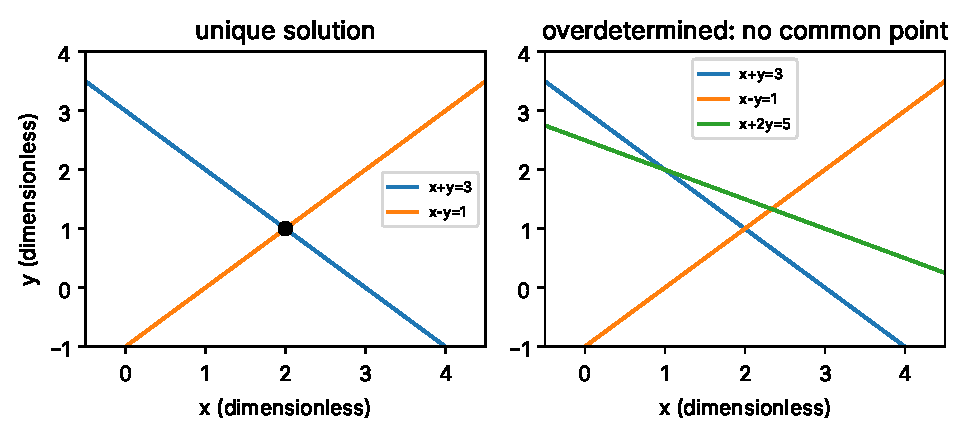
\includegraphics[width=0.85\linewidth]{figs/linear-algebra_lines.pdf}
\caption{Row picture of linear systems in two unknowns. Left: two equations $x+y=3$ and $x-y=1$ meet in exactly one point $(2,1)$. Right: adding a third equation $x+2y=5$ makes the system overdetermined; the three lines do not pass through a common point, so no exact solution exists. (Two parallel lines, not shown, would give either no solution or, if they coincide, infinitely many.) Axes dimensionless.}
\label{fig:linear-algebra-lines}
\end{figure}

\subsection{Row operations}

We record the system as the \emph{augmented matrix} $[A\,|\,\bm b]$ and apply three \emph{row operations}:
\begin{enumerate}
\item swap two equations;
\item multiply an equation by a nonzero number $s$;
\item add $s$ times one equation to another.
\end{enumerate}
\emph{Row operations do not change the set of solutions.} For (1) the equations are unchanged, only reordered. For (2), any $\bm x$ satisfying the old equation satisfies the new one (multiply by $s$), and conversely (divide by $s\ne0$). For (3), if $\bm x$ satisfies equations $i$ and $j$ it satisfies ``equation $j$ plus $s$ times equation $i$''; conversely, from the new system subtract $s$ times equation $i$ to recover the old equation $j$. Each operation is reversible, so no solution is gained or lost.

\subsection{Gaussian elimination and back substitution}

\emph{Gaussian elimination} uses operation (3) to clear the entries below the diagonal, one column at a time. In column 1, pick a row with a nonzero entry (the \emph{pivot}); swap it to the top if needed; subtract multiples of it from the rows below to make their column-1 entries zero. Then repeat with column 2 on the remaining rows, and so on. The result is an \emph{echelon} (staircase) form, upper triangular for a square system, which is solved from the bottom up by \emph{back substitution}.

\begin{sample}{Elimination on a $3\times3$ system}
Solve
\[
x+y+z=6,\qquad 2x+3y+z=11,\qquad x+2y+3z=14 .
\]

\textbf{Step 1:} Augmented matrix
$\left[\begin{array}{ccc|c}1&1&1&6\\2&3&1&11\\1&2&3&14\end{array}\right]$.

\textbf{Step 2:} Pivot $1$ in row 1. $R_2\leftarrow R_2-2R_1$: $(0,\,1,\,-1\,|\,-1)$. $R_3\leftarrow R_3-R_1$: $(0,\,1,\,2\,|\,8)$.

\textbf{Step 3:} Pivot $1$ in row 2, column 2. $R_3\leftarrow R_3-R_2$: $(0,\,0,\,3\,|\,9)$. The system is now
$\left[\begin{array}{ccc|c}1&1&1&6\\0&1&-1&-1\\0&0&3&9\end{array}\right]$.

\textbf{Step 4 (back substitution):} $3z=9\Rightarrow z=3$. Then $y-z=-1\Rightarrow y=2$. Then $x+y+z=6\Rightarrow x=6-2-3=1$.

\textbf{Step 5 (check):} $1+2+3=6$, $2+6+3=11$, $1+4+9=14$.
\[
\boxed{(x,y,z)=(1,2,3).}
\]
\end{sample}

\subsection{How much work is elimination?}

Count multiply-and-add operations for an $n\times n$ system. At step $k$ (clearing column $k$, $k=1,\dots,n-1$) there are $n-k$ rows below the pivot; each needs its $n-k$ remaining entries and its right-hand side updated, $n-k+1$ multiply-adds per row. The total is
\[
\sum_{k=1}^{n-1}(n-k)(n-k+1)=\sum_{j=1}^{n-1}j(j+1)\quad(j=n-k).
\]
Using $\sum_{j=1}^{n-1}j^2=\frac{(n-1)n(2n-1)}6$ and $\sum_{j=1}^{n-1}j=\frac{(n-1)n}2$,
\begin{equation}
\sum_{j=1}^{n-1}j(j+1)=\frac{(n-1)n(2n-1)}6+\frac{3(n-1)n}6=\frac{(n-1)n(2n+2)}6=\frac{(n-1)n(n+1)}3\approx\frac{n^3}3 .
\label{eq:linear-algebra-cost}
\end{equation}
For $n=3$ this gives $8$, which you can confirm by counting Step~2 ($2$ rows $\times$ $3$ updates) and Step~3 ($1\times2$) of the sample. Back substitution adds only about $n^2/2$. The $n^3$ growth matters: a dense $6000\times6000$ system needs about $7.2\times10^{10}$ multiply-adds. But if most entries are zero, the count collapses. For a \emph{tridiagonal} matrix (nonzero only on the diagonal and its two neighbors) each elimination step touches one row and two entries, so the work grows only like $n$. The paper's Hamiltonian is tridiagonal (Sec.~II~B, App.~A step~4), and Chapter~\ref{ch:eigen} explains how the same structure makes its eigenvalues cheap.

\begin{pycode}
import numpy as np
A = np.array([[1., 1, 1], [2, 3, 1], [1, 2, 3]])
b = np.array([6., 11, 14])
x = np.linalg.solve(A, b)        # elimination (LU) inside LAPACK
print(x)                         # [1. 2. 3.]
print(np.abs(A @ x - b).max())   # residual at rounding level
print(np.linalg.matrix_rank(A), np.linalg.det(A))   # 3, 3.0
\end{pycode}

\begin{keyideas}
\item Row operations are reversible and preserve the solution set.
\item Elimination to echelon form plus back substitution solves $A\bm x=\bm b$; the cost is $\approx n^3/3$ multiply-adds for a dense $n\times n$ system (\cref{eq:linear-algebra-cost}), far less for sparse (e.g.\ tridiagonal) ones.
\end{keyideas}

%======================================================================
\section{Rank, and systems with too many or too few equations}\label{sec:linear-algebra-rank}

\subsection{Pivots, free variables and rank}

Run elimination on any $m\times n$ matrix (swapping rows when a column has no usable pivot, and moving on to the next column if a whole column below the current row is zero). The result is an echelon form: each nonzero row starts with a pivot, strictly to the right of the pivot above it, and any all-zero rows are at the bottom.

\paragraph{Definitions.} The number $r$ of pivots is the \emph{rank} of $A$. Unknowns whose columns contain a pivot are \emph{pivot variables}; the other $n-r$ unknowns are \emph{free variables}.

\begin{beyond}
\textbf{Taken on trust: rank is well defined.} Different sequences of row operations can give different echelon forms, but they always have the same number of pivots. Moreover the rank equals the largest number of linearly independent columns of $A$, and also the largest number of independent rows (``row rank equals column rank''). Proofs: Strang \cite{strang}, Ch.~3; Trefethen and Bau \cite{trefethen}, Lecture~1.
\end{beyond}

Since there is at most one pivot per row and one per column, $r\le\min(m,n)$.

\paragraph{The three outcomes.} After elimination, consider each all-zero row of the left side. Its equation reads $0=\beta$, where $\beta$ is whatever the right-hand side has become.
\begin{itemize}
\item If some such $\beta\neq0$, there is \textbf{no solution} (the system is \emph{inconsistent}).
\item Otherwise there is at least one solution: assign the free variables any values and solve for the pivot variables by back substitution. If $r=n$ there are no free variables and the solution is \textbf{unique}. If $r<n$, each choice of the $n-r$ free variables gives a different solution, so there are \textbf{infinitely many}.
\end{itemize}

\subsection{The null space and the general solution}

The \emph{null space} of $A$ is the set of all $\bm x$ with $A\bm x=\bm 0$. It always contains $\bm 0$, and it is closed under linear combinations: if $A\bm x=\bm 0$ and $A\bm y=\bm 0$ then $A(\alpha\bm x+\beta\bm y)=\alpha A\bm x+\beta A\bm y=\bm 0$. By the discussion above (with $\bm b=\bm 0$, which is always consistent), its members are described by $n-r$ free parameters, so it is a subspace of dimension $n-r$.

If $\bm x_p$ is any one solution of $A\bm x=\bm b$ (a \emph{particular} solution) and $\bm x$ is another, then $A(\bm x-\bm x_p)=\bm b-\bm b=\bm 0$, so $\bm x-\bm x_p$ is in the null space. Hence
\begin{equation}
\bm x=\bm x_p+\bm x_h,\qquad A\bm x_h=\bm 0 ,
\label{eq:linear-algebra-general}
\end{equation}
is the general solution: one particular solution plus anything in the null space.

\subsection{Overdetermined and underdetermined systems}

\paragraph{Overdetermined ($m>n$, more equations than unknowns).} At most $n$ pivots, so at least $m-n$ rows of the echelon form are zero on the left. Each gives a condition $0=\beta$ that the right side must satisfy. For a generic right side, especially one containing measurement noise, these conditions fail and there is no exact solution (\cref{fig:linear-algebra-lines}, right). The sensible question becomes ``which $\bm x$ makes $A\bm x$ \emph{closest} to $\bm b$?'', which is least squares (Chapter~\ref{ch:least-squares}), the projection of \cref{eq:linear-algebra-closest}.

\paragraph{Underdetermined ($m<n$, fewer equations than unknowns).} At most $m$ pivots, so at least $n-m$ free variables. If the system is consistent at all, it has infinitely many solutions. If moreover $r=m$ (every equation has a pivot), there are no zero rows, so it is consistent for \emph{every} $\bm b$: the columns can combine into any target. An underdetermined model of full rank can therefore reproduce \emph{any} data exactly, and infinitely many coefficient vectors do so.

\begin{checkpoint}
A system has 400 equations and 600 unknowns. Can it have exactly one solution?
\end{checkpoint}
\checkanswer{No. The rank is at most 400, so there are at least $600-400=200$ free variables. Either there is no solution or there are infinitely many.}

\begin{sample}{Recovering zeros from spacings}
Given only the three spacings $\bm g=(6.887315,\,3.988818,\,5.414018)$, find all $\bm t\in\mathbb R^4$ with $D\bm t=\bm g$, where $D$ is the spacing matrix of the earlier sample.

\textbf{Step 1:} $D$ is already in echelon form, with pivots $-1$ in columns 1, 2, 3. So $r=3$, $n=4$, and $t_4$ is free. Three equations, four unknowns: underdetermined, consistent for every $\bm g$.

\textbf{Step 2:} Set $t_4=s$. Back substitution: $-t_3+t_4=g_3\Rightarrow t_3=s-g_3$; $-t_2+t_3=g_2\Rightarrow t_2=s-g_2-g_3$; $-t_1+t_2=g_1\Rightarrow t_1=s-g_1-g_2-g_3$.

\textbf{Step 3:} In the form \cref{eq:linear-algebra-general}:
\[
\bm t=(-g_1-g_2-g_3,\ -g_2-g_3,\ -g_3,\ 0)+s\,(1,1,1,1).
\]
The null space is spanned by $(1,1,1,1)$: shifting every zero by the same amount leaves all spacings unchanged.

\textbf{Step 4:} With $g_1+g_2+g_3=16.290151$ and the choice $s=t_4=30.424876$, $t_1=30.424876-16.290151=14.134725$, the true first zero.
\[
\boxed{\bm t=\bm t_p+s(1,1,1,1);\quad s=30.424876\ \Rightarrow\ t_1=14.134725.}
\]
Spacings alone cannot tell you where the zeros sit; one extra fact (one zero) is needed.
\end{sample}

\begin{keyideas}
\item Rank $r$ = number of pivots $\le\min(m,n)$; there are $n-r$ free variables.
\item General solution = particular solution + null space (\cref{eq:linear-algebra-general}).
\item Overdetermined systems usually have no exact solution (least squares instead); underdetermined systems of full row rank have infinitely many exact solutions for \emph{any} right side.
\end{keyideas}

%======================================================================
\section{The determinant}\label{sec:linear-algebra-det}

\subsection{The $2\times2$ determinant as an area}

Let the columns of $A=\begin{pmatrix}a_1&b_1\\a_2&b_2\end{pmatrix}$ be $\bm a=(a_1,a_2)$ and $\bm b=(b_1,b_2)$. The parallelogram they span has area $\abs{\bm a}\abs{\bm b}\sin\theta$. Square it and use $\sin^2\theta=1-\cos^2\theta$:
\begin{align*}
\text{area}^2&=\abs{\bm a}^2\abs{\bm b}^2-\abs{\bm a}^2\abs{\bm b}^2\cos^2\theta=\abs{\bm a}^2\abs{\bm b}^2-(\bm a\cdot\bm b)^2\\
&=(a_1^2+a_2^2)(b_1^2+b_2^2)-(a_1b_1+a_2b_2)^2\\
&=a_1^2b_1^2+a_1^2b_2^2+a_2^2b_1^2+a_2^2b_2^2-a_1^2b_1^2-2a_1b_1a_2b_2-a_2^2b_2^2\\
&=a_1^2b_2^2-2a_1b_2\,a_2b_1+a_2^2b_1^2\\
&=(a_1b_2-a_2b_1)^2 .
\end{align*}
So the area is $\abs{a_1b_2-a_2b_1}$, and we define the \emph{determinant}
\begin{equation}
\det\begin{pmatrix}a_1&b_1\\a_2&b_2\end{pmatrix}=a_1b_2-b_1a_2 ,
\label{eq:linear-algebra-det2}
\end{equation}
the same $ad-bc$ that appeared in the inverse. Its sign records orientation: positive if turning from $\bm a$ to $\bm b$ is counterclockwise.

Since $A\bm e_1=\bm a$ and $A\bm e_2=\bm b$, the map $A$ sends the unit square (spanned by $\bm e_1,\bm e_2$, area 1) to the parallelogram spanned by $\bm a,\bm b$. \emph{The determinant is the factor by which $A$ scales areas} (\cref{fig:linear-algebra-map}). If $\det A=0$ the parallelogram is flattened onto a line: the columns are parallel (dependent), and some nonzero vector is squashed to $\bm 0$, which is the singular case of \cref{sec:linear-algebra-inverse}.

\begin{figure}[htbp]\centering
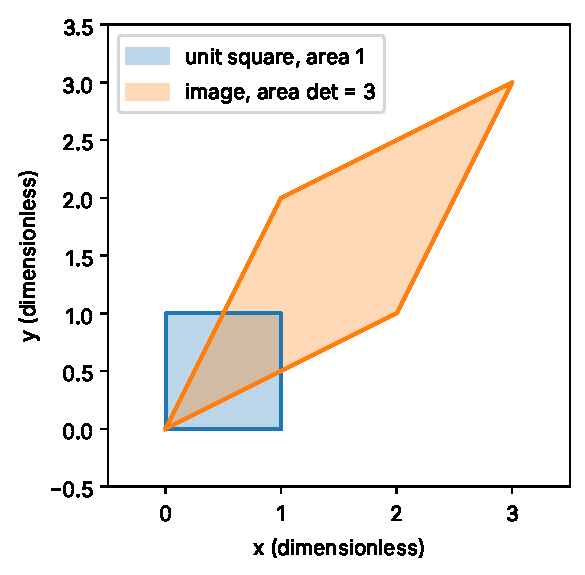
\includegraphics[width=0.85\linewidth]{figs/linear-algebra_map.pdf}
\caption{The matrix $\begin{pmatrix}2&1\\1&2\end{pmatrix}$ sends the unit square (area 1) to the parallelogram spanned by its columns $(2,1)$ and $(1,2)$, whose area is $\det=2\cdot2-1\cdot1=3$. Axes dimensionless.}
\label{fig:linear-algebra-map}
\end{figure}

\subsection{The $3\times3$ determinant as a volume}

For a $3\times3$ matrix, expand along the first row:
\begin{equation}
\det A=A_{11}(A_{22}A_{33}-A_{23}A_{32})-A_{12}(A_{21}A_{33}-A_{23}A_{31})+A_{13}(A_{21}A_{32}-A_{22}A_{31}).
\label{eq:linear-algebra-det3}
\end{equation}
Each bracket is the $2\times2$ determinant left after deleting the row and column of the entry in front, and the signs alternate $+,-,+$. Recall from first-year physics that the cross product of the second and third rows $\bm r_2,\bm r_3$ is $\bm r_2\times\bm r_3=(A_{22}A_{33}-A_{23}A_{32},\ A_{23}A_{31}-A_{21}A_{33},\ A_{21}A_{32}-A_{22}A_{31})$. Dotting with the first row $\bm r_1=(A_{11},A_{12},A_{13})$ reproduces \cref{eq:linear-algebra-det3} term by term (the middle term's sign is absorbed because $A_{23}A_{31}-A_{21}A_{33}=-(A_{21}A_{33}-A_{23}A_{31})$). So $\det A=\bm r_1\cdot(\bm r_2\times\bm r_3)$, and $\abs{\det A}$ is the volume of the parallelepiped spanned by the rows.

\subsection{Properties}

\begin{beyond}
\textbf{Taken on trust: properties of determinants.} The determinant extends to $n\times n$ matrices, and:
(D1) $\det I=1$;
(D2) swapping two rows changes the sign;
(D3) multiplying one row by $s$ multiplies $\det$ by $s$;
(D4) adding a multiple of one row to another leaves $\det$ unchanged;
(D5) the determinant of a triangular matrix is the product of its diagonal entries;
(D6) $\det(AB)=\det A\,\det B$;
(D7) $\det A^\top=\det A$;
(D8) $\det A\neq0$ if and only if $A$ is invertible, if and only if its rank is $n$.
Proofs: Strang \cite{strang}, Ch.~5; Riley, Hobson and Bence \cite{rhb}, Ch.~8. You can check any of them on small cases. For instance (D4) for $2\times2$: $\det\begin{pmatrix}a&b\\c+sa&d+sb\end{pmatrix}=a(d+sb)-b(c+sa)=ad-bc$.
\end{beyond}

\begin{checkpoint}
Use (D2) to show that a matrix with two equal rows has determinant zero.
\end{checkpoint}
\checkanswer{Swapping the two equal rows leaves the matrix unchanged, so its determinant is unchanged; by (D2) it also changes sign. So $\det=-\det$, which forces $\det=0$.}

Properties (D2), (D4), (D5) give a fast way to compute determinants: eliminate to triangular form, keep track of row swaps, and multiply the pivots.

\begin{sample}{A $3\times3$ determinant two ways}
Compute $\det A$ for $A=\begin{pmatrix}1&1&1\\2&3&1\\1&2&3\end{pmatrix}$, the matrix of the elimination sample.

\textbf{Step 1 (expansion, \cref{eq:linear-algebra-det3}):} $1\cdot(3\cdot3-1\cdot2)-1\cdot(2\cdot3-1\cdot1)+1\cdot(2\cdot2-3\cdot1)=7-5+1=3$.

\textbf{Step 2 (elimination):} The sample used only operations of type (D4) and reached $\begin{pmatrix}1&1&1\\0&1&-1\\0&0&3\end{pmatrix}$. By (D4) the determinant is unchanged; by (D5) it is $1\cdot1\cdot3=3$.
\[
\boxed{\det A=3\neq0,\ \text{so } A \text{ is invertible and the solution } (1,2,3) \text{ is unique.}}
\]
\end{sample}

For an $n\times n$ matrix, repeated expansion like \cref{eq:linear-algebra-det3} has $n!$ terms ($n!$ grows faster than any power), while elimination needs $\approx n^3/3$ operations. Computers always use elimination.

\begin{keyideas}
\item $\abs{\det A}$ is the area (2D) or volume (3D) scaling factor of $A$; $\det A=0$ means the columns are dependent and $A$ is singular.
\item Compute determinants by elimination: product of pivots, with a sign flip per row swap.
\end{keyideas}

%======================================================================
\section{Functions as vectors}\label{sec:linear-algebra-functions}

\subsection{Sampling a function on a grid}

A computer cannot store a function $f(x)$; it stores numbers. The paper (Sec.~II~B, App.~A step~3) works on the interval $(-L,L)$ with $N$ equally spaced \emph{interior} points,
\begin{equation}
x_j=-L+jh,\qquad j=1,\dots,N,\qquad h=\frac{2L}{N+1},
\label{eq:linear-algebra-grid}
\end{equation}
so the walls $x_0=-L$ and $x_{N+1}=L$ are not stored (the wavefunction is zero there, Chapter~\ref{ch:bound-states}). The function becomes the vector
\[
\bm f=(f(x_1),\,f(x_2),\,\dots,\,f(x_N))\in\mathbb R^N .
\]
(Here $N$ is the grid size; the same letter is used for zero-counting functions elsewhere, and context distinguishes them.) Adding functions or multiplying them by constants corresponds exactly to adding or scaling their sample vectors, so the sampled functions behave like vectors in $\mathbb R^N$ (\cref{fig:linear-algebra-grid}).

\begin{figure}[htbp]\centering
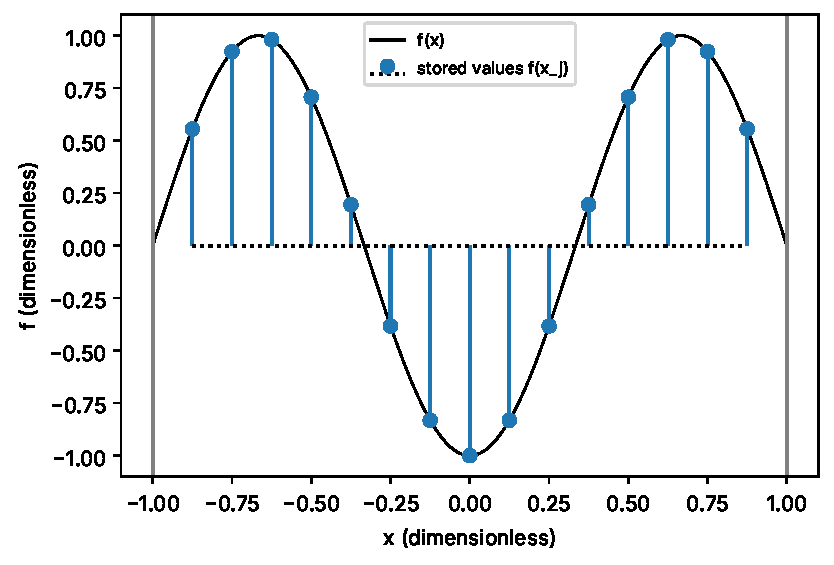
\includegraphics[width=0.85\linewidth]{figs/linear-algebra_grid.pdf}
\caption{A function as a vector. The curve $f(x)=\sin(3\pi(x+1)/2)$ on $(-1,1)$ is stored as its values (stems) at $N=15$ interior grid points $x_j=-1+jh$, $h=2/16$. The walls $x=\pm1$ (vertical lines), where $f=0$, are not stored. $x$ and $f$ dimensionless.}
\label{fig:linear-algebra-grid}
\end{figure}

\subsection{The inner product of functions}

For two sampled functions, the inner product of their vectors, multiplied by the spacing $h$, is
\[
h\sum_{j=1}^Nf(x_j)^*g(x_j),
\]
a Riemann sum for $\int f^*g\,\dd x$. As $h\to0$ (more and more points) it tends to the integral, by the definition of the integral as a limit of Riemann sums, for continuous $f$ and $g$. This motivates the definition
\begin{equation}
\langle f,g\rangle=\int_{-L}^{L}f(x)^*\,g(x)\,\dd x,\qquad \norm{f}=\sqrt{\langle f,f\rangle}=\sqrt{\int_{-L}^{L}\abs{f(x)}^2\dd x}.
\label{eq:linear-algebra-finner}
\end{equation}
It has the same four properties as \cref{eq:linear-algebra-cinner} (conjugate symmetry, linearity, conjugate-linearity, positivity), each proved the same way with the sum replaced by an integral. Positivity needs one remark: $\int\abs{f}^2\dd x=0$ forces $f=0$ for a continuous $f$, since a continuous non-negative function with zero integral must vanish everywhere. A function with $\norm{f}=1$ is \emph{normalized}; the paper normalizes its discrete eigenvectors by $\sum_j\psi_j^2\,h=1$ (App.~A step~9), the grid version of $\int\abs{\psi}^2\dd x=1$.

\begin{sample}{A grid sum that is exact}
Take $L=1$, $f(x)=\cos(\pi x/2)$ (which vanishes at the walls). Compute $h\sum_jf(x_j)^2$ for $N=3$, and show it equals $\int_{-1}^1f^2\dd x$ for every $N$.

\textbf{Step 1 ($N=3$):} $h=2/4=0.5$, points $-0.5,0,0.5$. Values of $f^2$: $\cos^2(\pi/4)=0.5$, $1$, $0.5$. Sum $2$, times $h$: $1$.

\textbf{Step 2 (exact integral):} $\int_{-1}^1\cos^2(\pi x/2)\dd x=\int_{-1}^1\tfrac12(1+\cos\pi x)\dd x=1+0=1$.

\textbf{Step 3 (any $N$):} With $x_j=-1+jh$, $h=2/(N+1)$: $\pi x_j/2=-\pi/2+j\pi/(N+1)$, and $\cos(\theta-\pi/2)=\sin\theta$, so $f(x_j)^2=\sin^2\frac{j\pi}{N+1}=\frac12\big(1-\cos\frac{2\pi j}{N+1}\big)$.

\textbf{Step 4:} Let $z=e^{2\pi i/(N+1)}$ (Chapter~\ref{ch:complex}). The finite geometric sum $S=\sum_{j=0}^Nz^j$ satisfies $zS-S=z^{N+1}-1=e^{2\pi i}-1=0$; since $z\ne1$ for $N\ge1$, $S=0$. Its real part gives $\sum_{j=0}^N\cos\frac{2\pi j}{N+1}=0$, so $\sum_{j=1}^N\cos\frac{2\pi j}{N+1}=-1$ (removing the $j=0$ term, which is $1$).

\textbf{Step 5:} $\sum_{j=1}^N f(x_j)^2=\frac12\big(N-(-1)\big)=\frac{N+1}2$, and times $h=\frac2{N+1}$ gives $1$.
\[
\boxed{h\sum_{j=1}^Nf(x_j)^2=1=\int_{-1}^1f^2\,\dd x\ \text{ for every } N.}
\]
\end{sample}

\begin{pitfall}
The interior-point sum omits the walls. That is harmless for functions that vanish there (wavefunctions in a box, and products involving them), but not in general. For $f=1$, $g=x^2$ on $(-1,1)$, the exact $\langle f,g\rangle=2/3\approx0.6667$, while $h\sum x_j^2=0.48$ for $N=9$ and $0.6468$ for $N=99$; the shortfall is about $h$ times the wall value $1$. Adding the two wall points with weight $h/2$ each (the trapezoid rule) removes most of it.
\end{pitfall}

\subsection{An orthogonal basis of cosines}

Consider the functions $\phi_k(x)=\cos(k\pi x/L)$, $k=0,1,2,\dots$, on $[-L,L]$, the basis the paper uses for $\delta V$ (Sec.~II~C). We show they are mutually orthogonal under \cref{eq:linear-algebra-finner}.

First, for an integer $q\ne0$,
\[
\int_{-L}^{L}\cos\frac{q\pi x}{L}\dd x=\frac{L}{q\pi}\Big[\sin\frac{q\pi x}{L}\Big]_{-L}^{L}=\frac{L}{q\pi}\big(\sin q\pi-\sin(-q\pi)\big)=0,
\]
and for $q=0$ the integrand is $1$, giving $2L$. Now use $\cos A\cos B=\tfrac12[\cos(A-B)+\cos(A+B)]$:
\begin{equation}
\langle\phi_j,\phi_k\rangle=\frac12\int_{-L}^{L}\cos\frac{(j-k)\pi x}{L}\dd x+\frac12\int_{-L}^{L}\cos\frac{(j+k)\pi x}{L}\dd x .
\label{eq:linear-algebra-cosprod}
\end{equation}
\begin{itemize}
\item $j\ne k$ (both $\ge0$): $j-k\ne0$ and $j+k\ne0$, so both integrals vanish: $\langle\phi_j,\phi_k\rangle=0$.
\item $j=k\ge1$: the first integral is $2L$, the second ($q=2k\ne0$) vanishes: $\langle\phi_k,\phi_k\rangle=L$.
\item $j=k=0$: $\phi_0=1$, and $\langle\phi_0,\phi_0\rangle=2L$.
\end{itemize}
Summarizing,
\begin{equation}
\int_{-L}^{L}\cos\frac{j\pi x}{L}\cos\frac{k\pi x}{L}\dd x=\begin{cases}0,&j\ne k,\\ L,&j=k\ge1,\\ 2L,&j=k=0.\end{cases}
\label{eq:linear-algebra-cosorth}
\end{equation}
They are orthogonal but not normalized; dividing $\phi_k$ by $\sqrt L$ (or $\phi_0$ by $\sqrt{2L}$) would make them orthonormal.

\subsection{Expanding a function in a basis}

Suppose an even function can be written as $f(x)=\sum_ka_k\phi_k(x)$. Take the inner product with $\phi_j$ and use \cref{eq:linear-algebra-cosorth}:
\[
\langle\phi_j,f\rangle=\sum_ka_k\langle\phi_j,\phi_k\rangle=a_j\langle\phi_j,\phi_j\rangle ,
\]
so
\begin{equation}
a_0=\frac1{2L}\int_{-L}^{L}f(x)\,\dd x,\qquad a_k=\frac1L\int_{-L}^{L}f(x)\cos\frac{k\pi x}L\,\dd x\quad(k\ge1).
\label{eq:linear-algebra-coeffs}
\end{equation}
This is \cref{eq:linear-algebra-components} for functions.

\begin{beyond}
\textbf{Taken on trust: completeness.} For an infinite sum, moving $\langle\phi_j,\cdot\rangle$ inside the sum, and the claim that every reasonable even function on $[-L,L]$ \emph{can} be written as $\sum_ka_k\cos(k\pi x/L)$, both need convergence theorems for Fourier series. They hold for continuous, piecewise-smooth even functions (convergence in the mean-square sense for much wider classes). See Riley, Hobson and Bence \cite{rhb}, Ch.~12, and Chapter~\ref{ch:fourier-series}. The paper never needs the infinite sum: it uses a finite $M$, for which no convergence question arises.
\end{beyond}

\begin{sample}{Cosine coefficients of $x^2$}
Expand $f(x)=x^2$ on $[-1,1]$ ($L=1$) in $\cos(k\pi x)$. Find $a_0,a_1,a_2,a_3$ and the partial sums at $x=0$.

\textbf{Step 1:} $a_0=\frac12\int_{-1}^1x^2\dd x=\frac12\cdot\frac23=\frac13$.

\textbf{Step 2:} For $k\ge1$, $a_k=\int_{-1}^1x^2\cos(k\pi x)\dd x$. Integrate by parts with $u=x^2$, $\dd v=\cos(k\pi x)\dd x$, $v=\sin(k\pi x)/(k\pi)$:
\[
a_k=\Big[\frac{x^2\sin k\pi x}{k\pi}\Big]_{-1}^1-\frac2{k\pi}\int_{-1}^1x\sin(k\pi x)\dd x=0-\frac2{k\pi}\int_{-1}^1x\sin(k\pi x)\dd x ,
\]
since $\sin(\pm k\pi)=0$.

\textbf{Step 3:} Again by parts, $u=x$, $\dd v=\sin(k\pi x)\dd x$, $v=-\cos(k\pi x)/(k\pi)$:
\[
\int_{-1}^1x\sin(k\pi x)\dd x=\Big[-\frac{x\cos k\pi x}{k\pi}\Big]_{-1}^1+\frac1{k\pi}\int_{-1}^1\cos(k\pi x)\dd x .
\]
The last integral is zero. At $x=1$ the bracket is $-(-1)^k/(k\pi)$; at $x=-1$ it is $-(-1)\cos(-k\pi)/(k\pi)=(-1)^k/(k\pi)$. Upper minus lower: $-2(-1)^k/(k\pi)$.

\textbf{Step 4:} $a_k=-\frac{2}{k\pi}\cdot\Big(-\frac{2(-1)^k}{k\pi}\Big)=\frac{4(-1)^k}{k^2\pi^2}$. So $a_1=-4/\pi^2=-0.40528$, $a_2=1/\pi^2=0.10132$, $a_3=-4/(9\pi^2)=-0.04503$.

\textbf{Step 5:} At $x=0$ every $\cos(0)=1$. Partial sums: $a_0+a_1=-0.0720$; $+a_2$: $0.0294$; $+a_3$: $-0.0157$. They approach the true value $0$, overshooting alternately.
\[
\boxed{a_0=\tfrac13,\quad a_k=\frac{4(-1)^k}{k^2\pi^2}\ (k\ge1).}
\]
\end{sample}

\begin{figure}[htbp]\centering
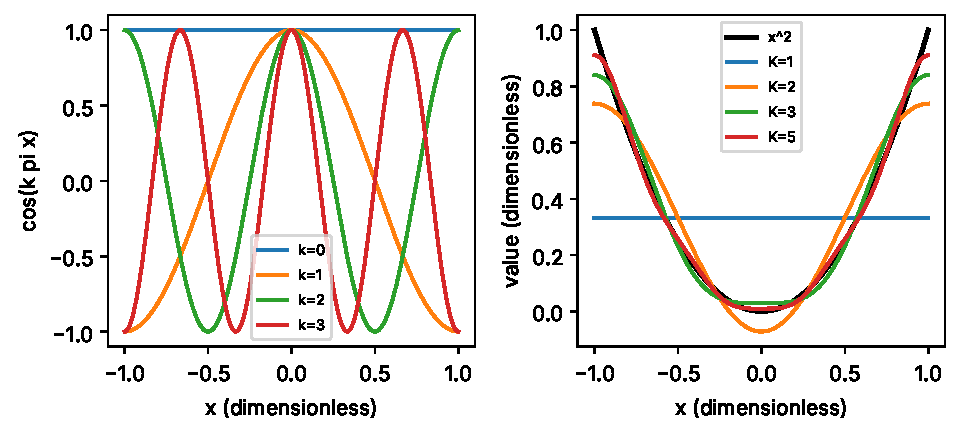
\includegraphics[width=0.85\linewidth]{figs/linear-algebra_cosine.pdf}
\caption{Left: the first cosine basis functions $\cos(k\pi x/L)$, $k=0,1,2,3$, on $[-L,L]$ with $L=1$; they are mutually orthogonal (\cref{eq:linear-algebra-cosorth}). Right: $x^2$ (black) and its partial cosine sums with $K=1,2,3,5$ terms ($k=0,\dots,K-1$), using $a_0=1/3$, $a_k=4(-1)^k/(k^2\pi^2)$. $x$ and function values dimensionless.}
\label{fig:linear-algebra-cosine}
\end{figure}

\subsection{Non-orthogonal bases}

The paper also uses Chebyshev polynomials $T_k(2|x|/L-1)$ and piecewise-linear ``hat'' functions (Sec.~II~C, ``Other bases''; Chapter~\ref{ch:fitting} defines them). Under $\int\dd x$ these are not mutually orthogonal (neighboring hats overlap, for instance). The coefficients are then no longer single inner products. If $f=\sum_ka_k\phi_k$ exactly, taking the inner product with each $\phi_j$ gives
\begin{equation}
\sum_k\underbrace{\langle\phi_j,\phi_k\rangle}_{G_{jk}}a_k=\underbrace{\langle\phi_j,f\rangle}_{b_j}\qquad\Longleftrightarrow\qquad G\bm a=\bm b ,
\label{eq:linear-algebra-gram}
\end{equation}
a linear system with the \emph{Gram matrix} $G$. For an orthogonal basis $G$ is diagonal and \cref{eq:linear-algebra-gram} collapses to \cref{eq:linear-algebra-coeffs}; otherwise you solve it by elimination. (When $f$ is \emph{not} exactly in the span, the same equations give the closest function in the span, the least-squares fit of Chapter~\ref{ch:least-squares}; Problem~17 is an example.)

\begin{keyideas}
\item On the grid $x_j=-L+jh$, $h=2L/(N+1)$, a function is a vector in $\mathbb R^N$; $h\sum f_j^*g_j\to\int f^*g\,\dd x$.
\item $\cos(k\pi x/L)$ are orthogonal on $[-L,L]$ (\cref{eq:linear-algebra-cosorth}); expansion coefficients are inner products (\cref{eq:linear-algebra-coeffs}).
\item For non-orthogonal bases, coefficients solve the Gram system $G\bm a=\bm b$ (\cref{eq:linear-algebra-gram}).
\end{keyideas}

%======================================================================
\section{A matrix made of integrals: the sensitivity matrix}\label{sec:linear-algebra-sens}

In the paper (Sec.~II~C), the energy levels $E_n$ of a quantum particle in a potential $V(x)$ are adjusted by adding a correction $\delta V(x)=\sum_{k=0}^{M-1}c_k\phi_k(x)$. Chapter~\ref{ch:perturbation} derives that, to first order, each level moves by
\begin{equation}
\delta E_n\approx\sum_{k=0}^{M-1}A_{nk}\,c_k,\qquad A_{nk}=\int_{-L}^{L}\abs{\psi_n(x)}^2\phi_k(x)\,\dd x ,
\label{eq:linear-algebra-Ank}
\end{equation}
where $\psi_n$ is the normalized wavefunction of level $n$ ($\int\abs{\psi_n}^2\dd x=1$). Here we take \cref{eq:linear-algebra-Ank} as given and study it as linear algebra. (The paper also uses the letter $A$ for a non-Hermitian operator in Sec.~II~E; that is a different object.)

\paragraph{Reading the matrix.} Row $n$ belongs to level $n$, column $k$ to basis function $k$. In the column picture \cref{eq:linear-algebra-colpic}, $\delta\bm E=A\bm c$ is a combination of columns: column $k$ is the pattern of level shifts produced by basis function $k$ at unit amplitude. Entry $A_{nk}$ is the inner product $\langle\abs{\psi_n}^2,\phi_k\rangle$ of two real functions: the overlap between where level $n$ ``lives'' and the shape of basis function $k$.

\paragraph{The first column is all ones.} With $\phi_0=1$, $A_{n0}=\int\abs{\psi_n}^2\dd x=1$ for every $n$, by normalization alone, for any potential. So a constant correction $c_0$ shifts every level by the same $c_0$, to first order. This is the ``joint shift'' direction, and it will matter in Chapter~\ref{ch:non-hermitian}, where a constant imaginary potential produces no real shift at all.

\paragraph{On a grid.} With $W_{nj}=\abs{\psi_n(x_j)}^2$ (an $n_{\rm lev}\times N$ matrix) and $\Phi_{jk}=\phi_k(x_j)$ (an $N\times M$ matrix), the Riemann sum for \cref{eq:linear-algebra-Ank} is
\begin{equation}
A_{nk}\approx h\sum_{j=1}^NW_{nj}\Phi_{jk}=h\,(W\Phi)_{nk},
\label{eq:linear-algebra-AWPhi}
\end{equation}
a single matrix product, \cref{eq:linear-algebra-matmul}.

\begin{sample}{The sensitivity matrix of the box}
For an infinite square well on $[-L,L]$ (running example RE3), Chapter~\ref{ch:bound-states} shows the normalized states are $\psi_n(x)=\frac1{\sqrt L}\sin\frac{n\pi(x+L)}{2L}$, $n=1,2,\dots$. Compute $A_{nk}$ for the cosine basis.

\textbf{Step 1 (square):} $\abs{\psi_n}^2=\frac1L\sin^2\theta$ with $\theta=\frac{n\pi(x+L)}{2L}$. Using $\sin^2\theta=\frac12(1-\cos2\theta)$ and $2\theta=\frac{n\pi x}L+n\pi$,
\[
\abs{\psi_n}^2=\frac1{2L}\Big[1-\cos\Big(\frac{n\pi x}{L}+n\pi\Big)\Big].
\]

\textbf{Step 2:} $\cos(\alpha+n\pi)=\cos\alpha\cos n\pi-\sin\alpha\sin n\pi=(-1)^n\cos\alpha$. So
\[
\abs{\psi_n}^2=\frac1{2L}\Big[1-(-1)^n\cos\frac{n\pi x}{L}\Big]=\frac1{2L}\big[\phi_0-(-1)^n\phi_n\big].
\]

\textbf{Step 3:} $A_{nk}=\langle\abs{\psi_n}^2,\phi_k\rangle=\frac1{2L}\big[\langle\phi_0,\phi_k\rangle-(-1)^n\langle\phi_n,\phi_k\rangle\big]$. Apply \cref{eq:linear-algebra-cosorth} with $n\ge1$: for $k=0$, $\frac1{2L}[2L-0]=1$; for $k\ge1$, $\frac1{2L}[0-(-1)^nL\,\delta_{nk}]$.
\[
\boxed{A_{nk}=\begin{cases}1,&k=0,\\ (-1)^{n+1}/2,&k=n,\\ 0,&\text{otherwise}.\end{cases}}
\]
Every row has the $1$ in column $0$ and at most one more nonzero entry, $+\frac12$ for odd $n$ and $-\frac12$ for even $n$. Remarkably, the answer does not depend on $L$.
\end{sample}

The box matrix is extremely sparse. For the Wu--Sprung potential that the paper uses (Chapter~\ref{ch:wu-sprung}), the wavefunctions are not pure sines, and $A$ fills in (\cref{fig:linear-algebra-Amatrix}). The bookkeeping, however, is identical, and the box lets us see the rank questions of \cref{sec:linear-algebra-rank} by hand.

\begin{figure}[htbp]\centering
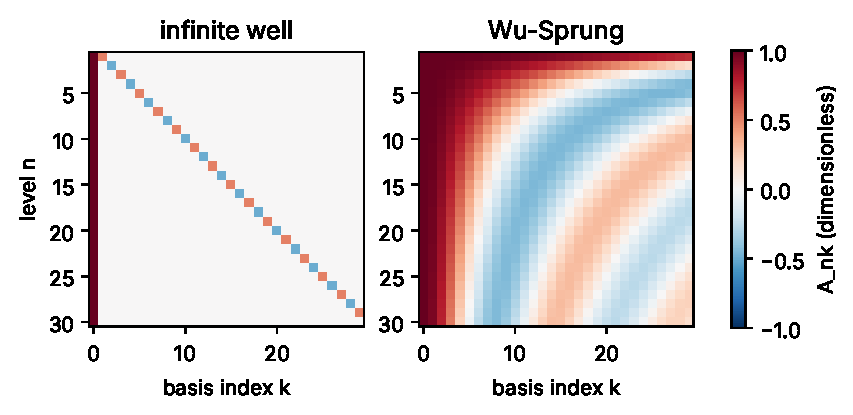
\includegraphics[width=0.85\linewidth]{figs/linear-algebra_Amatrix.pdf}
\caption{Sensitivity matrices $A_{nk}=\int\abs{\psi_n}^2\cos(k\pi x/L)\,\dd x$ for the first 30 levels ($n$, rows) and 30 cosines ($k$, columns), with $L=44.883$ (scale 1). Left: infinite square well, from the formula of the box sample (first column $1$, diagonal $\pm\frac12$). Right: Wu--Sprung potential, computed on a 1200-point finite-difference grid; the first column is again $1$, but the rest of the matrix is no longer sparse. Entries are dimensionless.}
\label{fig:linear-algebra-Amatrix}
\end{figure}

\begin{sample}{Too many and too few coefficients in the box}
Take three box levels with target shifts $\bm r=(0.2,\,-0.1,\,0.3)$. (a) With $M=4$ coefficients $c_0,\dots,c_3$, find all exact solutions of $A\bm c=\bm r$. (b) With $M=2$ ($c_0,c_1$), show there is no exact solution.

\textbf{Step 1 (a):} From the box formula, rows $n=1,2,3$, columns $k=0,\dots,3$:
\[
A=\begin{pmatrix}1&\tfrac12&0&0\\ 1&0&-\tfrac12&0\\ 1&0&0&\tfrac12\end{pmatrix}.
\]
Three equations, four unknowns: underdetermined.

\textbf{Step 2 (a):} Choose $c_0=s$ as the free variable. Row 1: $s+c_1/2=0.2\Rightarrow c_1=2(0.2-s)$. Row 2: $s-c_2/2=-0.1\Rightarrow c_2=2(0.1+s)$. Row 3: $s+c_3/2=0.3\Rightarrow c_3=2(0.3-s)$.

\textbf{Step 3 (a):} In the form \cref{eq:linear-algebra-general}: $\bm c=(0,\,0.4,\,0.2,\,0.6)+s(1,-2,2,-2)$. Check the null vector: $A(1,-2,2,-2)=(1-1,\ 1-1,\ 1-1)=\bm 0$. Raising $c_0$ lifts all three levels, and the other three coefficients exactly cancel it.

\textbf{Step 4 (b):} Now $A=\begin{pmatrix}1&\tfrac12\\1&0\\1&0\end{pmatrix}$. Rows 2 and 3 say $c_0=-0.1$ and $c_0=0.3$. Elimination ($R_3\leftarrow R_3-R_2$) gives the row $0=0.4$: inconsistent.
\[
\boxed{\text{(a) } \bm c=(0,0.4,0.2,0.6)+s(1,-2,2,-2),\ s\in\mathbb R;\qquad \text{(b) no solution.}}
\]
With $M=2$ levels 2 and 3 are reachable only through $c_0$, so their different targets cannot both be met; with $M=4$ every level has its own coefficient plus a spare, and infinitely many coefficient vectors fit perfectly.
\end{sample}

\begin{checkpoint}
For the box with $n_{\rm lev}$ levels and $M=n_{\rm lev}+1$ coefficients ($k=0,\dots,n_{\rm lev}$), what is the rank of $A$, and what is the dimension of its null space?
\end{checkpoint}
\checkanswer{Columns $1,\dots,n_{\rm lev}$ are $\pm\frac12$ times the standard basis vectors, which are independent and span $\mathbb R^{n_{\rm lev}}$, so the rank is $n_{\rm lev}$. The null space has dimension $M-n_{\rm lev}=1$, spanned by the vector that combines column 0 with the others to cancel, as in the sample.}

\begin{pycode}
import numpy as np
L, N = 44.883, 3000                 # RE3 box, scale-1 half-width
h = 2*L/(N + 1)
x = -L + h*np.arange(1, N + 1)      # interior grid points
nlev, M = 6, 6
n = np.arange(1, nlev + 1)          # levels start at 1
k = np.arange(M)                    # cosines start at 0
psi = np.sin(np.outer(x + L, n)*np.pi/(2*L))/np.sqrt(L)   # N x nlev
Phi = np.cos(np.outer(x, k)*np.pi/L)                       # N x M
A = h*(psi**2).T @ Phi              # nlev x M, the grid version of A_nk
print(np.round(A, 6))               # first column 1, A[n-1, n] = +-0.5
\end{pycode}

\begin{keyideas}
\item The paper's $A_{nk}=\int\abs{\psi_n}^2\phi_k\,\dd x$ is a matrix of inner products: rows are levels, columns are basis functions; on a grid it is $h\,W\Phi$.
\item Its first column is all ones for any potential: $c_0$ shifts every level equally.
\item For the box, $A$ is sparse and the over/underdetermined cases can be solved by hand.
\end{keyideas}

%======================================================================
\section{Paper connection}\label{sec:linear-algebra-paper}

Here is where the tools of this chapter appear in the paper \cite{soniR1} (revision R1; code and data in \cite{zenodo}).

\paragraph{The correction as a basis expansion (Sec.~II~C).} The fitted correction $\delta V(x)=\sum_{k=0}^{M-1}c_k\cos(k\pi x/L)$ is a finite expansion in the orthogonal cosine basis of \cref{eq:linear-algebra-cosorth}; the vector $c\in\mathbb R^M$ is everything the fit can adjust. The ``Other bases'' paragraph replaces the cosines by Chebyshev polynomials and hat functions, which are not orthogonal under $\int\dd x$; the Gram system \cref{eq:linear-algebra-gram} shows that the coefficients of a non-orthogonal basis are coupled to one another. Only the basis changes; the vector bookkeeping is the same.

\paragraph{The sensitivity matrix and the residual vector (Sec.~II~C, App.~A step~6).} The paper forms the residual vector $r$ with components $r_n=\tilde t_n-E_n$ and the matrix $A_{nk}=\int\abs{\psi_n}^2\cos(k\pi x/L)\,\dd x$, then updates $c$ by a damped least-squares solution of $A\,\delta c\approx r$. The shape of $A$ is (number of training levels)$\times M$. In Table~I, the scale-1 fit on zeros 1--400 with $M=200$ has a $400\times200$ matrix (overdetermined); the same fit with $M=600$ has $400\times600$ (underdetermined, null space of dimension at least $200$). The first column is all ones (\cref{sec:linear-algebra-sens}), so $c_0$ moves all levels together. The ``SVD-damped'' step itself is the subject of Chapter~\ref{ch:least-squares}; the update rule as a whole is explained in Chapter~\ref{ch:fitting}.

\paragraph{``More coefficients than levels''.} \Cref{sec:linear-algebra-rank} showed that an underdetermined system of full row rank has exact solutions for \emph{every} right-hand side, and infinitely many of them. This is the linear-algebra core of several statements in the paper. Sec.~III reports that on the full 500 zeros the fit reaches rms $0.186$ at $M=300$ and reproduces all 500 zeros to rms $<10^{-4}$ spacings by $M=900$. Table~III notes that the odd/even splits have 200 training levels at scale 1, ``so the rows with $M\ge200$ are saturated'', and the $M=400$ odd/even rows indeed have in-sample error $<10^{-3}$. Sec.~IV says of control B that ``at 900 coefficients on 400 zeros the least-squares problem is underdetermined''. (Control B's model $F(t)=\sum_j[a_j\sin(\omega_jt)+b_j\cos(\omega_jt)]$ is linear in the amplitudes, so its fit is literally a linear system with one row per training zero and one column per coefficient: 150 primes times three harmonics times two amplitudes gives 900 columns; control C1 has 450 frequencies times two, again 900.) A caution about status: the operator fit is nonlinear, because $\psi_n$ and $E_n$ change as $c$ changes, so the counting argument applies exactly only to each linearized step. The paper's own statement is empirical and heuristic: the bases ``are effectively complete for in-sample level patterns, so they realize essentially arbitrary joint shifts'' (Sec.~VI). The surrogate tests of Sec.~III, in which shuffled and phase-randomized targets are fitted as well as the true zeros (in-sample rms $0.134\pm0.010$, $0.141\pm0.006$, $0.138\pm0.005$ against $0.137$ for the true zeros), are what a nearly full-rank, nearly saturated linear model would lead you to expect.

\paragraph{rms is a norm; corr is an angle.} Every rms in the paper is $\norm{\bm e}/\sqrt n$ for an error vector measured in local mean spacings (\cref{eq:linear-algebra-rms}). The null rms on the principal holdout, zeros 401--500 (running example RE5), is $0.2631$ (App.~A, key anchors), so the null error vector over those 100 zeros has norm $0.2631\times\sqrt{100}=2.631$. The correlations are the cosines of \cref{eq:linear-algebra-corr}. The geometry of \cref{eq:linear-algebra-beatnull} explains why the paper can say both ``the held-out rms never improves on the null'' and ``no reproducible positive held-out correlation appears'' (Sec.~III): with $\cos\theta\lesssim0$ no nonzero prediction can beat the null. Fig.~1 shows the two extremes, the fitted operator with held-out correlation $-0.07$ and the six-prime formula with $+0.96$. As a rough consistency check only (it assumes mean-zero vectors and optimal amplitude, and the correlation is rounded to two digits), \cref{eq:linear-algebra-sintheta} with $\cos\theta=0.96$ gives a best error of $0.263\times\sqrt{1-0.96^2}=0.074$ spacings, the same as the six-prime rms $0.074$ reported for 401--500 in Table~V.

\paragraph{Functions on grids (Sec.~II~B, App.~A steps 3, 4, 9).} At scale 1 the paper uses $L=44.8827$ and a working grid of $N=6000$ interior points, so every wavefunction is a vector in $\mathbb R^{6000}$ with spacing $h=2L/(N+1)\approx0.01496$ (\cref{eq:linear-algebra-grid}). Eigenvectors are normalized by $\sum\psi^2\,\dd x=1$, the grid form of $\norm{\psi}=1$ (step~9). The Hamiltonian matrix is real symmetric and tridiagonal (step~4: diagonal $2/\dd x^2+V$, off-diagonal $-1/\dd x^2$); Chapters~\ref{ch:eigen} and~\ref{ch:finite-differences} take it from there.

\paragraph{Vector identities.} The no-leakage argument, Eq.~(3), $\tilde t_n-E_n[\mathrm{fit}]=t_n-(E_n[\mathrm{fit}]-\Delta_n)$, is an identity between vectors: subtracting the fixed vector $\Delta$ from the targets is the same as adding it to the prediction. Eq.~(5), $\delta E_n=-c^\top T^{(n)}c$, is a quadratic form, one $M\times M$ matrix $T^{(n)}$ per level. The sum rule of Sec.~V~A, $\sum_n\delta E_n=0$, says that the vector of second-order shifts is orthogonal to the all-ones vector $(1,\dots,1)$.

\paragraph{Complex vectors and overlaps (Sec.~II~E).} In the non-Hermitian study the eigenvectors of $H+iA$ are complex, and they are ``matched to the unperturbed basis by overlap'': the overlap is the complex inner product \cref{eq:linear-algebra-cinner}, whose modulus is largest for the unperturbed state the perturbed one most resembles (Chapters~\ref{ch:eigen} and~\ref{ch:non-hermitian}). Notice the overloaded symbols: $A$ is the sensitivity matrix in Sec.~II~C but a non-Hermitian multiplication operator in Sec.~II~E; $N$ is the grid size in App.~A but the zero-counting function in Eq.~(1).

%======================================================================
\section{Summary}\label{sec:linear-algebra-summary}

\begin{itemize}
\item Vectors in $\mathbb R^n$ and $\mathbb C^n$ are ordered lists; addition and scaling act componentwise (\cref{eq:linear-algebra-add,eq:linear-algebra-scale}).
\item Real inner product $\bm u\cdot\bm v=\sum u_jv_j$ (\cref{eq:linear-algebra-dot}); complex $\langle\bm u,\bm v\rangle=\sum u_j^*v_j$ (\cref{eq:linear-algebra-cinner}); norm $\norm{\bm v}=\sqrt{\langle\bm v,\bm v\rangle}$; rms $=\norm{\bm e}/\sqrt n$ (\cref{eq:linear-algebra-rms}).
\item Cauchy--Schwarz $\abs{\bm u\cdot\bm v}\le\norm{\bm u}\norm{\bm v}$ (\cref{eq:linear-algebra-cs}) defines angles (\cref{eq:linear-algebra-angle}); correlation is the cosine between centered vectors (\cref{eq:linear-algebra-corr}); a prediction beats the null iff $\norm{\bm p}<2\norm{\bm d}\cos\theta$ (\cref{eq:linear-algebra-beatnull}); best rescaled error $\norm{\bm d}\sin\theta$ (\cref{eq:linear-algebra-sintheta}).
\item Orthonormal components are inner products (\cref{eq:linear-algebra-components}); $\norm{\bm v}^2=\sum\abs{a_k}^2$ (\cref{eq:linear-algebra-parseval}); projection gives the closest point (\cref{eq:linear-algebra-projsub,eq:linear-algebra-closest}).
\item Matrices are linear maps; $A\bm x$ is a combination of columns (\cref{eq:linear-algebra-colpic}); $(AB)_{ik}=\sum_jA_{ij}B_{jk}$ (\cref{eq:linear-algebra-matmul}); $(AB)^\top=B^\top A^\top$; $\langle\bm u,A\bm v\rangle=\langle A^\dagger\bm u,\bm v\rangle$ (\cref{eq:linear-algebra-adjoint}).
\item $2\times2$ inverse (\cref{eq:linear-algebra-inv2}) exists iff $ad-bc\ne0$; elimination solves $A\bm x=\bm b$ in $\approx n^3/3$ operations (\cref{eq:linear-algebra-cost}).
\item Rank = number of pivots; general solution = particular + null space (\cref{eq:linear-algebra-general}); overdetermined systems usually have no exact solution, underdetermined full-rank systems have infinitely many for every right side.
\item Determinants: area/volume factors (\cref{eq:linear-algebra-det2,eq:linear-algebra-det3}); $\det A\ne0$ iff invertible.
\item Functions as grid vectors (\cref{eq:linear-algebra-grid}); $\langle f,g\rangle=\int f^*g\,\dd x$ (\cref{eq:linear-algebra-finner}); cosine orthogonality (\cref{eq:linear-algebra-cosorth}); coefficients (\cref{eq:linear-algebra-coeffs}); Gram system for non-orthogonal bases (\cref{eq:linear-algebra-gram}).
\item Sensitivity matrix $A_{nk}=\int\abs{\psi_n}^2\phi_k\,\dd x$ (\cref{eq:linear-algebra-Ank}), first column all ones; on a grid $A\approx hW\Phi$ (\cref{eq:linear-algebra-AWPhi}).
\end{itemize}

%======================================================================
\section{Problems}\label{sec:linear-algebra-problems}

\begin{problemlist}
\prob{1}{For $\bm u=(2,-1,3,0)$ and $\bm v=(1,4,0,-2)$, compute $\bm u+\bm v$, $3\bm u-2\bm v$, $\bm u\cdot\bm v$, $\norm{\bm u}$ and $\norm{\bm v}$.}
\prob{1}{Normalize $\bm w=(1,2,2)$.}
\prob{1}{A fit leaves residuals $(0.1,\,-0.2,\,0.2,\,0.0,\,-0.1)$ in mean spacings. What is the rms?}
\prob{1}{For $\bm u=(i,\,1+2i)$ and $\bm w=(1,\,i)$, compute $\norm{\bm u}$, $\norm{\bm w}$ and $\langle\bm u,\bm w\rangle$, and verify Cauchy--Schwarz.}
\prob{2}{Prove that if $\bm u\cdot\bm v=0$ then $\norm{\bm u+\bm v}^2=\norm{\bm u}^2+\norm{\bm v}^2$, and conversely, for real vectors, that this equality implies $\bm u\cdot\bm v=0$.}
\prob{1}{Compute $A\bm x$ for $A=\begin{pmatrix}2&1\\0&3\\1&-1\end{pmatrix}$ and $\bm x=(1,2)$, using both the row and the column picture.}
\prob{2}{Compute $AB$ and $BA$ for $A=\begin{pmatrix}1&2\\3&4\end{pmatrix}$, $B=\begin{pmatrix}0&1\\1&0\end{pmatrix}$. Describe in words what multiplying by $B$ on the left and on the right does.}
\prob{2}{Prove $(AB)^\dagger=B^\dagger A^\dagger$ for complex matrices, using indices.}
\prob{1}{Find the inverse of $\begin{pmatrix}3&1\\5&2\end{pmatrix}$ and check it.}
\prob{2}{Solve by elimination: $2x+y-z=1$, $x+3y+2z=13$, $3x-y+z=4$.}
\prob{2}{For the system $x+2y=3$, $2x+ay=b$, find the values of $a$ and $b$ for which there is (i) a unique solution, (ii) no solution, (iii) infinitely many solutions.}
\prob{2}{Find the rank of $\begin{pmatrix}1&2&3\\2&4&6\\1&0&1\end{pmatrix}$ and a vector spanning its null space.}
\prob{1}{Compute $\det\begin{pmatrix}2&0&1\\1&3&2\\1&1&1\end{pmatrix}$. What does your answer say about the columns?}
\prob{1}{Find the area of the parallelogram spanned by $(3,1)$ and $(1,2)$.}
\prob{2}{Compute $\int_{-L}^{L}\cos^2(3\pi x/L)\,\dd x$, $\int_{-L}^{L}\cos(\pi x/L)\cos(2\pi x/L)\,\dd x$ and $\int_{-L}^{L}\sin(\pi x/L)\cos(\pi x/L)\,\dd x$.}
\prob{2}{Find the cosine coefficients of $f(x)=\abs{x}$ on $[-1,1]$ ($L=1$). Evaluate the partial sum with $k=0,1$ at $x=0$.}
\prob{3}{The functions $1$ and $x$ on $[0,1]$ are not orthogonal. Set up and solve the Gram system \cref{eq:linear-algebra-gram} with $f(x)=x^2$, using $\langle f,g\rangle=\int_0^1fg\,\dd x$. Interpret the resulting function $a_0+a_1x$.}
\prob{2}{(Paper.) App.~A step~3 of the paper gives the working grids: $L=44.8827$, $N=6000$ at scale 1, and $L=59.9572$, $N=8000$ at scale 2. Compute the grid spacing $h$ at each scale and state the length of the vector storing one wavefunction.}
\prob{2}{(Paper.) Give the shape of the sensitivity matrix for these configurations of Tables I and III, and say whether each linearized system is over- or underdetermined and the minimum dimension of the null space when underdetermined: (a) scale 1, fit 1--300, $M=400$; (b) scale 1, fit 1--400, $M=200$; (c) scale 2, fit 1--800, $M=900$; (d) the scale-1 odd split with $M=400$. Relate (d) to the in-sample entry in Table~III.}
\prob{2}{(Paper.) Table~V reports, on held-out zeros 401--500, a null rms of $0.263$ and rms $0.074$ (six primes) and $0.043$ (25 primes). Convert each into the norm of the error vector over those 100 zeros, and give the ratio of the null norm to the six-prime norm.}
\prob{3}{Prove the Cauchy--Schwarz inequality $\abs{\langle\bm u,\bm v\rangle}\le\norm{\bm u}\norm{\bm v}$ for complex vectors. (Hint: expand $\norm{\bm u-\lambda\bm v}^2$ with complex $\lambda=\langle\bm v,\bm u\rangle/\norm{\bm v}^2$.)}
\prob{2}{Prove that for any normalized $\psi_n$, the column $k=0$ of $A_{nk}$ (with $\phi_0=1$) is all ones. What does this imply for the first-order effect of adding a constant to the potential?}
\prob{2}{(Computational.) Using numpy, build the box sensitivity matrix on a grid as in the last listing of \cref{sec:linear-algebra-sens} (with $L=44.883$, $N=3000$, six levels, six cosines) and compare it with the analytic result of the box sample. How large is the largest deviation?}
\prob{2}{(Computational.) Using \texttt{numpy.linalg.matrix\_rank}, find the ranks of the two box matrices of the sample ``Too many and too few coefficients in the box''. Then use \texttt{numpy.linalg.solve} on a random $5\times5$ system and print the largest component of $A\bm x-\bm b$.}
\prob{3}{(Computational, paper.) Using qmnt, form the vector of fluctuations $d_n=(t_n-s_n)/\gap_n$ for $n=401,\dots,500$ with \texttt{qmnt.zeros} and \texttt{qmnt.fluct}, and compute its rms. Compare with the paper's null (App.~A, key anchors). Explain why the rms of $\bm d$ is the null's error.}
\prob{2}{Compute the Pearson correlation of $\bm p=(1,2,3,4)$ and $\bm d=(2,1,4,3)$ using \cref{eq:linear-algebra-corr}.}
\prob{3}{Derive \cref{eq:linear-algebra-cost} for the operation count of elimination, verify it for $n=3$, and evaluate it for $n=6000$. Why is a tridiagonal system so much cheaper?}
\prob{3}{Project $\bm v=(1,2,3)$ onto the plane spanned by the orthonormal vectors $\bm e_1=(1,0,0)$ and $\bm e_2=(0,1,1)/\sqrt2$, and check that the residual is orthogonal to the plane.}
\prob{2}{Show that the rotation matrix $R(\theta)=\begin{pmatrix}\cos\theta&-\sin\theta\\ \sin\theta&\cos\theta\end{pmatrix}$ preserves lengths and has determinant 1.}
\prob{3}{(Paper.) In control B of the paper (Sec.~II~D and Sec.~IV, Table~IV), the fluctuation is modeled as $F(t)=\sum_j[a_j\sin(\omega_jt)+b_j\cos(\omega_jt)]$ with $\omega_j=m\log p$ for 150 primes and $m=1,2,3$, fitted to 400 training zeros. Write the fitting problem as a linear system, give the shape of its matrix, the minimum null-space dimension, and explain why ridge regularization (Chapter~\ref{ch:least-squares}) is needed to pick a single answer.}
\prob{3}{Among all solutions $\bm c=(0,0.4,0.2,0.6)+s(1,-2,2,-2)$ of part (a) of the box sample, find the one with the smallest norm. Show that it is orthogonal to the null vector $(1,-2,2,-2)$, and explain geometrically why it must be.}
\end{problemlist}

%======================================================================
\section{Answers to selected problems}\label{sec:linear-algebra-answers}

\textbf{Problem 1.} Componentwise: $\bm u+\bm v=(3,3,3,-2)$; $3\bm u-2\bm v=(6-2,\,-3-8,\,9-0,\,0+4)=(4,-11,9,4)$; $\bm u\cdot\bm v=2-4+0+0=-2$; $\norm{\bm u}=\sqrt{4+1+9}=\sqrt{14}=3.7417$; $\norm{\bm v}=\sqrt{1+16+4}=\sqrt{21}=4.5826$.

\textbf{Problem 2.} $\norm{\bm w}=\sqrt{1+4+4}=3$, so $\hat{\bm w}=(1/3,\,2/3,\,2/3)$, whose norm is $\sqrt{(1+4+4)/9}=1$.

\textbf{Problem 3.} Squares $0.01+0.04+0.04+0+0.01=0.10$; divide by 5: $0.02$; square root: $\rms=0.1414$.

\textbf{Problem 4.} $\norm{\bm u}^2=\abs{i}^2+\abs{1+2i}^2=1+5=6$, $\norm{\bm u}=\sqrt6$; $\norm{\bm w}^2=1+1=2$. $\langle\bm u,\bm w\rangle=(-i)(1)+(1-2i)(i)=-i+i-2i^2=2$. Cauchy--Schwarz: $\abs{2}^2=4\le6\cdot2=12$.

\textbf{Problem 5.} $\norm{\bm u+\bm v}^2=(\bm u+\bm v)\cdot(\bm u+\bm v)=\norm{\bm u}^2+2\,\bm u\cdot\bm v+\norm{\bm v}^2$ by linearity and symmetry. If $\bm u\cdot\bm v=0$ the middle term vanishes. Conversely, if $\norm{\bm u+\bm v}^2=\norm{\bm u}^2+\norm{\bm v}^2$, the same expansion forces $2\,\bm u\cdot\bm v=0$.

\textbf{Problem 6.} Rows: $(2\cdot1+1\cdot2,\ 0+3\cdot2,\ 1-2)=(4,6,-1)$. Columns: $1\cdot(2,0,1)+2\cdot(1,3,-1)=(4,6,-1)$.

\textbf{Problem 7.} $AB=\begin{pmatrix}2&1\\4&3\end{pmatrix}$, $BA=\begin{pmatrix}3&4\\1&2\end{pmatrix}$. Multiplying by $B$ on the right swaps the columns of $A$; on the left it swaps the rows. So $AB\ne BA$.

\textbf{Problem 9.} $\det=6-5=1$, so by \cref{eq:linear-algebra-inv2} the inverse is $\begin{pmatrix}2&-1\\-5&3\end{pmatrix}$. Check: $\begin{pmatrix}3&1\\5&2\end{pmatrix}\begin{pmatrix}2&-1\\-5&3\end{pmatrix}=\begin{pmatrix}6-5&-3+3\\10-10&-5+6\end{pmatrix}=I$.

\textbf{Problem 11.} $\det=a-4$. (i) If $a\ne4$ the matrix is invertible: a unique solution for every $b$. (ii), (iii) If $a=4$, subtract twice the first equation from the second: $0=b-6$. So $a=4$, $b\ne6$ gives no solution; $a=4$, $b=6$ gives infinitely many ($x=3-2y$, $y$ free).

\textbf{Problem 13.} By \cref{eq:linear-algebra-det3}: $2(3\cdot1-2\cdot1)-0+1(1\cdot1-3\cdot1)=2-2=0$. The matrix is singular and its columns are dependent; indeed column 3 $=(1,2,1)=\tfrac12(2,1,1)+\tfrac12(0,3,1)$, half the sum of the first two.

\textbf{Problem 14.} Area $=\abs{3\cdot2-1\cdot1}=5$ (\cref{eq:linear-algebra-det2}).

\textbf{Problem 15.} By \cref{eq:linear-algebra-cosorth}: $L$ (case $j=k=3\ge1$) and $0$ (case $j\ne k$). For the third, $\sin\alpha\cos\alpha=\tfrac12\sin2\alpha$ and $\int_{-L}^{L}\sin(2\pi x/L)\,\dd x=0$ because the integrand is odd; so $0$.

\textbf{Problem 17.} $G=\begin{pmatrix}\int1&\int x\\ \int x&\int x^2\end{pmatrix}=\begin{pmatrix}1&1/2\\1/2&1/3\end{pmatrix}$, $\bm b=(\int x^2,\int x^3)=(1/3,1/4)$. $\det G=1/3-1/4=1/12$, so $G^{-1}=12\begin{pmatrix}1/3&-1/2\\-1/2&1\end{pmatrix}$ and $\bm a=12\,(1/9-1/8,\ -1/6+1/4)=12\,(-1/72,\ 1/12)=(-1/6,\ 1)$. The function $x-1/6$ is the straight line closest to $x^2$ in the norm $\sqrt{\int_0^1(\cdot)^2\dd x}$, since $x^2$ is not in the span of $\{1,x\}$ and the equations select its projection.

\textbf{Problem 19.} (a) $300\times400$: underdetermined, null space of dimension at least $100$. (b) $400\times200$: overdetermined. (c) $800\times900$: underdetermined, null space at least $100$. (d) $200\times400$: underdetermined, null space at least $200$; this is what Table~III calls ``saturated'', and its in-sample entry $<10^{-3}$ is what one expects when a nearly full-rank model has more coefficients than training levels. (The fit is nonlinear, so this counting is a guide, not a proof.)

\textbf{Problem 21.} If $\bm v=\bm 0$ both sides vanish. Otherwise, for complex $\lambda$, $0\le\norm{\bm u-\lambda\bm v}^2=\norm{\bm u}^2-\lambda\langle\bm u,\bm v\rangle-\lambda^*\langle\bm v,\bm u\rangle+\abs{\lambda}^2\norm{\bm v}^2$, using conjugate-linearity in the first slot and linearity in the second. Put $\lambda=\langle\bm v,\bm u\rangle/\norm{\bm v}^2$, so $\lambda^*=\langle\bm u,\bm v\rangle/\norm{\bm v}^2$. Then $\lambda\langle\bm u,\bm v\rangle=\lambda^*\langle\bm v,\bm u\rangle=\abs{\langle\bm u,\bm v\rangle}^2/\norm{\bm v}^2$ and $\abs{\lambda}^2\norm{\bm v}^2=\abs{\langle\bm u,\bm v\rangle}^2/\norm{\bm v}^2$. The inequality becomes $0\le\norm{\bm u}^2-\abs{\langle\bm u,\bm v\rangle}^2/\norm{\bm v}^2$; multiply by $\norm{\bm v}^2$ and take square roots.

\textbf{Problem 23.} Running the listing and subtracting the analytic matrix (first column $1$, entries $(-1)^{n+1}/2$ at $k=n$, zeros elsewhere) gives a largest deviation below $10^{-9}$, at the level of rounding errors. The agreement is this good because $\abs{\psi_n}^2\cos(k\pi x/L)$ vanishes at the walls and is a sum of a few cosines, for which the equally spaced sum over a full period is exact (the mechanism is the geometric-sum argument of the sample ``A grid sum that is exact'').

\textbf{Problem 25.} \texttt{d = qmnt.fluct(qmnt.zeros(500)[400:], np.arange(401, 501))} and \texttt{qmnt.rms(d)} give about $0.263$, matching the paper's null $0.2631$. The null predicts $t_n=s_n$, so its error vector in mean spacings is exactly $-\bm d$, and $\rms(-\bm d)=\rms(\bm d)$.

\textbf{Problem 27.} See \cref{eq:linear-algebra-cost}: $\sum_{j=1}^{n-1}j(j+1)=(n-1)n(n+1)/3$. For $n=3$: $2\cdot3\cdot4/3=8$, matching the count in the elimination sample. For $n=6000$: $5999\cdot6000\cdot6001/3\approx7.2\times10^{10}$. In a tridiagonal matrix each elimination step has a single nonzero below the pivot and only two entries to update, so the total grows like $n$, not $n^3$.

\textbf{Problem 29.} $\norm{R\bm x}^2=(x\cos\theta-y\sin\theta)^2+(x\sin\theta+y\cos\theta)^2=x^2(\cos^2\theta+\sin^2\theta)+y^2(\sin^2\theta+\cos^2\theta)+2xy(-\cos\theta\sin\theta+\sin\theta\cos\theta)=x^2+y^2$. $\det R=\cos^2\theta+\sin^2\theta=1$.

\textbf{Problem 31.} $\norm{\bm c}^2=s^2+(0.4-2s)^2+(0.2+2s)^2+(0.6-2s)^2$. Its derivative $2s-4(0.4-2s)+4(0.2+2s)-4(0.6-2s)=26s-3.2$ vanishes at $s=3.2/26=8/65\approx0.1231$, giving $\bm c\approx(0.1231,\ 0.1538,\ 0.4462,\ 0.3538)$. Its inner product with $(1,-2,2,-2)$ is $0.1231-0.3077+0.8923-0.7077=0$ (to rounding). Geometrically, the solutions form a line parallel to the null vector; by the closest-point argument \cref{eq:linear-algebra-closest}, the point of that line nearest the origin is where the line is perpendicular to the vector from the origin, so the minimum-norm solution has no component along the null space. Chapter~\ref{ch:least-squares} obtains it from the pseudo-inverse.
